% !TeX root = ADP-SG-Tester.tex

\chapter{Problem and Approaches to Solution}\label{ch:ProblemsMethods}

This chapter introduces the classical revenue management problem of capacity control problem under customer choice behaviour as can be found \eg in \cite{Koch.2017} or in \cite{Strauss.2018}. The problem consists of deciding which products to offer at a given point in time and \Cref{s:Prob} describes it in general as well as formulates it as a dynamic program. Various methods of solving the problem are laid out in \Cref{s:Metho}, before \Cref{s:ADP} introduces a more enhanced solution method, Approximate Dynamic Programming.

\section{The problem}\label{s:Prob}

This section describes the capacity control in general in \Cref{ss:Prob:GenDesc}, presents a concrete example in the airline setting in \Cref{ss:Prob:AirDesc} and introduces the formulation of the resulting choice based capacity control model as a dynamic program in \Cref{ss:Prob:FormDynProg}. \todo{Subsection zu Problemen in der Lösung einfügen, die überleitet zu den verschiedenen Lösungsmethoden}

\subsection{General description}\label{ss:Prob:GenDesc}

We cover a setting that is most regularly seen in every-day life: A company offers a bundle of products to heterogeneous customers arriving over time. Let us now introduce some terminology. \emph{Products} often correspond to services that have to be delivered at a given point in time. The period of time from now until delivery is referred to as \emph{selling horizon} (or booking horizon), is considered finite and is split into a finite set of consecutive \emph{time points}. The set of available products is also assumed to be finite and without loss of generality (w.\,l.\,o.\,g.\nomenclature{\wlogMath}{without loss of generality}) constant over time\footnote{If the set of available products change over time, let $S_t$ denote the set of available products at time $t$ and let $\mathcal{T}$ represent the finite set of time points. Then, $S \coloneqq \cup_{t \in \mathcal{T}}S_t$ is again finite (finite union of finite sets) and can be taken as the constant set of available products at each time point.}. Each individual product is characterized by a given \emph{price} and usage of certain, finitely many resources. These \emph{resources} might be shared among different products. 

The goal of business companies operating is to increase profits, which is equivalent to maximizing revenue. As stated, the price of individual products (leading to revenue) is assumed to be fixed, which is a realistic assumption for short terms considering potentially large costs coming with a change of price (\eg selling products via catalogue). Furthermore, capacities are fixed in the short term (costly to increase production as \eg more employees have to be hired) and are considered perishable. Often, capacity comes with high fixed costs and low marginal costs resulting from selling an additional product at any price (\eg costs for operating one flight with 97 customers are mostly the same as for operating the same flight with 98 customers). Such a profit and cost structure justify the usage of revenue as a proxy for profit as also stated in \cite{Strauss.2018}.

Switching to the customer side, the consideration of a heterogeneous customer group allows for modelling most real world scenarios. Not every customer is the same, but it is certainly reasonable to combine individuals to groups sharing similar characteristics. Some characteristics will be more prevalent in the overall population (more precise, the group of people that represents all persons interested in the companies' products).  Different customers have varying needs, thus different preferences and different willingness-to-pay, leading ultimately to different purchases depending on the currently offered set of products. Thus, the company can influence the sales process by altering the offered set of products over the booking horizon, which is exactly the task of capacity control under customer choice behaviour.

\subsection{Description in airline setting}\label{ss:Prob:AirDesc}

The concepts introduced above are now applied to a concrete airline setting, which will later be used to present the solution techniques. The airline company AirCo operates a flight network connecting cities A, B and C as depicted in \Cref{fig:AirDesc}. The booking horizon consists of 20 time steps (\eg today is Monday, booking is possible four times every day until and including Friday and flights depart on Saturday). The products to be offered are summarized in \Cref{tb:AirDesc:Prod}. Note that two products are available on Leg 1, \ie the expensive product 1 and the less expensive product 2 (\eg due to separate business and economy classes). A sell of either product 1 or product 2 will result in the reduction of available capacity on Leg 1 by one unit. Furthermore, product 6 presents an option to get from city A to city C (via city B) and thus a sell of product 6 results in a reduction of capacities on both Leg 1 and Leg 2 by one unit. Also product 4 is connecting city A and city C (on the direct flight) but is more expensive then product 6 (\eg the company assumes the shorter travel time is of value to some travellers). 

Furthermore, capacities are presented in \Cref{tb:AirDesc:Res}, so there are eight available seats on Leg 1, but just four seats are available on Leg 2. Customers are characterized as stated in \Cref{tb:AirDesc:Cust}, so most customers belong to segment 1 (higher value of $\lambda_l$ representing larger size of customer segment $l$), want to travel from city A to city B and prefer the budget option (as the value of preference for the latter product is much higher and a higher value corresponds to a higher preference). Customers belonging to segment 2 also want to travel from A to B, but are price insensitive, as they value the higher comfort of the more expensive product 1 just little higher as the cheaper product 2. Business customers that need to travel from A to C are represented by customer segment 3 as can be seen by the low preference for no-purchase. 

\todo{Idee: Beschreibung der Customer Segmente könnte man zu \enquote{Persona} ausweiten}
\begin{figure}
	\begin{subfigure}[t]{.3\linewidth}
		\centering
		\caption{Airline network. \label{fig:AirDesc}}
		\begin{tikzpicture}[
		mycircle/.style={
			circle,
			draw=black,
			fill=gray,
			fill opacity = 0.3,
			text opacity=1,
			inner sep=0pt,
			minimum size=20pt,
			font=\small},
		myarrow/.style={-Stealth},
		node distance=0.6cm and 1.2cm
		]
		\node[mycircle] (cB) {$B$};
		\node[mycircle,below left=of cB] (cA) {$A$};
		\node[mycircle,below right=of cB] (cC) {$C$};
		
		\foreach \i/\j/\txt/\p in {% start node/end node/text/position
			cA/cB/Leg 1/above,
			cB/cC/Leg 2/above}
		\draw [myarrow] (\i) -- node[sloped,font=\small,\p] {\txt} (\j);
		\draw[myarrow]([yshift= 20pt] cA) -- node[sloped,font=\small,above] {Leg 3} ([yshift= 20pt] cC);
		\draw[myarrow]([yshift= -20pt] cC) -- node[sloped,font=\small,below] {Leg 4} ([yshift= -20pt] cA);
		\end{tikzpicture}
	\end{subfigure}%
	\quad
	\begin{subtable}[t]{.4\linewidth}
		\caption{Products. \label{tb:AirDesc:Prod}}
		\small
		\centering
		\begin{tabular}{yxz}
			\toprule
			\text{Product} & \text{Origin-destination} & \text{Fare}\\
			\midrule
			1 & A \rightarrow B & 5\\
			2 & A \rightarrow B & 3\\
			3 & B \rightarrow C & 5\\
			4 & A \rightarrow C & 12\\
			5 & C \rightarrow A & 10\\
			6 & A \rightarrow B \rightarrow C & 8\\
			\bottomrule
		\end{tabular}
	\end{subtable}%
	\quad
	\begin{subtable}[t]{.2\linewidth}
		\caption{Resources. \label{tb:AirDesc:Res}}
		\small
		\centering
		\begin{tabular}{yy}
			\toprule
			\text{Leg} & \text{Capacity}\\
			\midrule
			1 & 8\\
			2 & 4\\
			3 & 4\\
			4 & 8\\
			\bottomrule
		\end{tabular}
	\end{subtable}
	
	\begin{subtable}{\linewidth}
		\caption{Customers.\label{tb:AirDesc:Cust}}
		\small
		\centering
		\begin{tabular}{lccccc}
			\toprule
			Seg. & $\lambda_l$ & \specialcell[b]{Consideration\\tuple\footnote{Note that in contrast to \cite{Bront.2009}, we use the mathematically correct terminology as \emph{tuple} does have an inherent order, while \emph{set} does not (and thus makes no mathematical sense to be combined with a preference vector referring to the order of products in the set).}} & \specialcell[b]{Preference \\vector} & \specialcell[b]{No purchase \\preference} & Description\\
			\midrule
			1 & $0.3$ & $(1, 2)$ & $(4, 8)$ & $2$ & Price sensitive, (A$\rightarrow$B)\\
			2 & $0.2$ & $(1, 2)$ & $(6, 5)$ & $2$ & Price insensitive, (A$\rightarrow$B)\\
			3 & $0.2$ & $(4, 6)$ & $(8, 4)$ & $1$ & Price sensitive, fast (A$\rightarrow$C)\\
			4 & $0.1$ & $(5)$ & $(2)$ & $2$ & Opportunity traveller, (C$\rightarrow$A)\\
			\bottomrule
		\end{tabular}
	\end{subtable}
	\caption{Working example to illustrate problem with $T=20$ time periods.}
\end{figure}


\subsection{Formulation as dynamic program}\label{ss:Prob:FormDynProg}


\todo{Übersichtsliteratur \cite{Phillips.2011} anschauen (nur an Uni Augsburg, nicht an TUM)}
Extensive literature deals with revenue management and came up with formal notation suitable for the analysis of capacity control models. Good overviews can be found in \cite{Klein.2008} or in \cite{Phillips.2011}. In this thesis, we introduce notation for a capacity control model first under a general discrete choice model of demand and then directly using a multinomial logit model of demand. Notation is closely linked to \cite{Koch.2017} and the standard representation is used for a better orientation with the main ideas outlined in \Cref{tb:Prob:Notation}\,.

\todo{Idee: Notation vereinheitlichen, stets ähnlich zu $t=1, \dots, T$. Also z.B. statt $j=1,\dots,n$ für Produkte auch $j=1,\dots,J$}
\begin{table}
	\begin{tabular}{cll}
		\toprule
		Symbol & Characteristic & Meaning\\
		\midrule
		$i, j, h, t, l, p$ & general small letter & index\\
		$n, m$ & specific small letters & maximum index\\
		$[n]$ & set of natural numbers& $\{1, \dots, n\}$\\
		$T, L$ & general capital letter & maximum index\\
		$S$ & specific capital letter & tuple of elements\\
		$x_1$ & small with index & single number\\
		$\boldsymbol{x}$ & small and bold & vector\\
		$(x_1, \dots, x_n)$ & parenthesis around single numbers & row vector\\
		$(\dots)^\intercal$ & $^\intercal$ on upper side & transpose\\
		\bottomrule
	\end{tabular}
	\caption{Concepts of notation}\label{tb:Prob:Notation}
\end{table}

\subsubsection{Formal notation}

First, we present the situation with its inflexible components. Consider a firm that produces $n$ distinguishable products indexed by $j = 1, \dots, n$. We introduce the notation $[n] \coloneqq \{1, \dots, n\}$. Product $j$ comes with a certain price leading to a revenue of $r_j$ when the product is sold. The revenues are bundled by the vector $\boldsymbol{r} = (r_1, \dots, r_n)^\intercal$. A total of $m$ distinct resources are used for production, which are indexed by  $h \in [m]$. In order to produce one unit of product $j$, certain resources are needed and the consumption of resources is captured by the vector $\boldsymbol{a}_j = (a_{1j}, \dots, a_{mj})^\intercal$ are necessary, with $a_{hj}=1$ if resource $h$ is needed for production of product $j$ and $a_{hj} = 0$ otherwise. The resource consumption can be aggregated in the incidence matrix $A = (a_{hj})_{h\in [m], j \in [n]}\in {0, 1}^{m \times n}$. Additionally, the firm already identified the group of potential customers and segmented this group into a total of $L$ customer segments, which are indexed by $l \in [L]$. A customer of segment $l$ arrives with probability $\lambda_l$ and this parameter can be adjusted such that it matches the reality (\eg there are two times as many customers belonging to segment $a$ then there are of segment $b$, so we choose $\lambda_a = 2\lambda_b$ ) and the model assumptions (only one customer arrives during each period).
\todo{Skalierung und Einflüsse auf Ankunftsraten in Fußnote oder Appendix}
\todo{Ergänzung: Beweis zu arrival probabilities können aufsummiert als kleiner gleich 1 angenommen werden, da der Parameter eines Poisson Prozesses dessen erwartete Ankunftszeit (? eig höher => mehr Leute kommen) beschreibt und damit mit der Feinheit der Zeitschritte angepasst werden kann. Poisson Prozess in \cite{Bront.2009} 3. Model
You just heard that the Poisson distribution is a limit of the Binomial distribution for rare events. This makes sense if you think about the stories. Say we do a Bernoulli trial every minute for an hour, each with a success probability of 0.1. We would do 60 trials, and the number of successes is Binomially distributed, and we would expect to get about 6 successes. This is just like the Poisson story we discussed in the video, where we get on average 6 hits on a website per hour. So, the Poisson distribution with arrival rate equal to np approximates a Binomial distribution for n Bernoulli trials with probability p of success (with n large and p small). Importantly, the Poisson distribution is often simpler to work with because it has only one parameter instead of two for the Binomial distribution.
The means are all about the same, which can be shown to be true by doing some pen-and-paper work. The standard deviation of the Binomial distribution gets closer and closer to that of the Poisson distribution as the probability p gets lower and lower. }. 

The finite time period from when booking is possible for the first time to when it is possible for the last time is discretized into a total of $T$ sufficiently small time periods, such that in each individual time period at most one customer arrives. Time periods are indexed by $t \in [T]$. To be very precise (particularly relevant for correct implementation), booking itself is just possible at the beginning of a time period, \ie for time period $t$, booking is possible at time point $t-1$. Furthermore, one customer purchases at most one product. 

Second, we look at the flexible components of the model, \ie those components that might change over time. Initially, \ie at the start of the first time period (time point 0), the available capacity of resource $h$ is given by $c_h^0$ and thus all available capacities are described by the vector $\boldsymbol{c}^0 = (c_1^0, \dots, c_m^0)^\intercal$. 

Let us now explore what happens if product $j$ is purchased during time period $t$, \ie at time point $t-1$. The old capacity vector is given by $\boldsymbol{c}^{t-1}$. As product $j$ claims capacities according to $\boldsymbol{a}_j$,  the capacity vector reduces accordingly to $\boldsymbol{c}^{t} = \boldsymbol{c}^{t-1} - \boldsymbol{a}_j$. Time moves forward, such that the last selling might occur at time period $T$, \ie at time point $T-1$.

The distinguishment of time period and time point is also visualized in \Cref{fig:Prob:Horizon} and one more comment on this topic: Time period $t$ can be seen as the following half open interval between time points: $(t-1, t]$.

\begin{figure}
	\centering
	\begin{tikzpicture}[snake=zigzag, line before snake = 5mm, line after snake = 5mm]
	% draw horizontal line   
	\draw (0,0) -- (2,0);
	\draw[snake] (2,0) -- (4,0);
	\draw (4,0) -- (6,0);
	\draw[snake] (6,0) -- (8,0);
	\draw (8,0) -- (9,0);
	
	% draw vertical lines
	\foreach \x in {0,1,2,4,5,6,8,9}
	\draw (\x cm,3pt) -- (\x cm,-3pt);
	
	% draw nodes
	\draw (0,0) node[below=3pt] {$ 0 $};
	\draw (0.5,0) node[above=3pt] {$ 1 $};
	\draw (1,0) node[below=3pt] {$ 1 $};
	\draw (1.5,0) node[above=3pt] {$ 2 $};
	\draw (2,0) node[below=3pt] {$ 2 $};
	
	\draw (4,0) node[below=3pt] {$ t-1 $};
	\draw (4.5,0) node[above=3pt] {$ t $};
	\draw (5,0) node[below=3pt] {$ t $};
	\draw (5.5,0) node[above=3pt] {$ t+1 $};
	\draw (6,0) node[below=3pt] {$ t+1 $};
	
	\draw (8,0) node[below=3pt] {$ T-1 $};
	\draw (8.5,0) node[above=3pt] {$ T $};
	\draw (9,0) node[below=3pt] {$ T $};
	
	\draw (11.3,0) node[below=3pt] {\parbox{3cm}{$\leftarrow~$ Time Point}} node[above=3pt] {\parbox{3cm}{$\leftarrow~$ Time Period}};
	\end{tikzpicture}
	\caption{Visualization of booking horizon with its time periods vs. its time points.\label{fig:Prob:Horizon}}
\end{figure}


To sum it up, the firm aims at increasing the value of the products sold and has flexibility in the sets offered. Thus, the decision variables for each time period $t \in [T]$ are given by $\boldsymbol{x}^t = (x^t_1, \dots, x^t_n)^\intercal$ with $x^t_j = 1$ if product $j$ is offered during time period $t$ (\ie chosen at time point $t-1$) and $x^t_j = 0$ otherwise. Thus, for each time period $t$ and the prevalent capacity $\boldsymbol{c}$, the offer set $\boldsymbol{x}$ has to be determined. Note that in machine learning terms, this mapping is defined as a policy $\boldsymbol{\psi}(\boldsymbol{c}, t)$.\todo{ML-Notation hier anfügen oder wo?}

We can put the goal mentioned above in formulas after introducing the random variable $X^t$ as the product which is purchased at time point $t$, with the notation $X^t=\{0\}$ if no-purchase is made at time point $t$. 
So we use $\Omega \coloneqq \{0, 1, \dots n\}$ as the underlying set (no-purchase plus all purchasable products) and can use $\mathcal{F} = \text{P}(\Omega)$ as underlying sigma algebra, with $\text{P}(\cdot)$ describing the power set\footnote{Note that $\text{P}(\Omega)$ is finite as $\Omega$ is finite by assumption}. 
Furthermore, we introduce a probability measure $p_{\boldsymbol{x}^t}(\cdot)$ 
and use the shorthand $p_{\boldsymbol{x}^t}(j) = p_{\boldsymbol{x}^t}(\{j\}) = p_{\boldsymbol{x}^t}(X^t = \{j\})$ as the probability of product $j$ being purchased at time point $t$ when tuple $\boldsymbol{x}^t$ is offered. Note that $p$ has to satisfy the corresponding Kolmogorov axioms, as it is a probability measure:
\begin{alignat}{2}
p_{\boldsymbol{x}^t}(j) &\geq 0 ~~\forall j \in \{1, \dots n\} \quad &&\text{(non-negativity)}\\
p_{\boldsymbol{x}^t}(\Omega) &= 1 &&\text{(unitarity)}\\
p_{\boldsymbol{x}^t}(\cup_{j \in J}\{j\}) &= \sum_{j \in J}p_{\boldsymbol{x}^t}(j) ~~\forall J \subset \Omega \quad &&\text{(additivity in discrete setting)}
\end{alignat}

How to arrive at those probabilities is discussed in \Cref{sss:DCM}. Now, we formalize the aim of the firm. The expected revenue-to-go starting with time period $t$ and capacity $\boldsymbol{c}$ is given by the value function $V(t, \boldsymbol{c})$, which maximizes the expected revenue and is mostly formulated recursively because of complicated evolutions due to capacities changing over time.

%todo Verbindung zu Erwartungswert herstellen
%&= \max_{x^t \in \{0,1\}^n}\left\{ \mathbb{E}_{\boldsymbol{x}^t}(r_{X^t})\right\}\\

\begin{align}
V(t, \boldsymbol{c}) &= \max_{x^t \in \{0,1\}^n}\left\{ \sum_{j \in [n]} p_{\boldsymbol{x}^t}(j) \left( r_j + V(t+1, \boldsymbol{c} - \boldsymbol{a}_j) \right) + p_{\boldsymbol{x}^t}(0) V(t+1, \boldsymbol{c}) \right\} \label{eq:Bellman}\\
&= \max_{x^t \in \{0,1\}^n}\left\{ \sum_{j \in [n]} p_{\boldsymbol{x}^t}(j) \left( r_j - \Delta_j V(t+1, \boldsymbol{c}) \right) \right\} + V(t+1, \boldsymbol{c}) ~\forall t \in [T], \boldsymbol{c} \geq 0
\end{align}

with $\Delta_j V(t+1, \boldsymbol{c}) \coloneqq V(t+1, \boldsymbol{c}) - V(t+1, \boldsymbol{c} - \boldsymbol{a}_j)$ and boundary conditions $V(T+1, \boldsymbol{c}) = 0$ if $\boldsymbol{c} \geq \boldsymbol{0}$ and $V(t, \boldsymbol{c}) = - \infty ~\forall t \in [T+1]$ if $\boldsymbol{c} \ngeq \boldsymbol{0}$, \ie $\exists h \in [m]: c_h < 0$\,.

Note that for determining the optimal offerset, the very last summand $V(t+1, \boldsymbol{c})$ is irrelevant for the maximization as it is constant over all offersets. The optimal offerset $\hat{\boldsymbol{x}}^t$ is thus given by

\begin{align}
\hat{\boldsymbol{x}}^t = \argmax_{x^t \in \{0,1\}^n}\left\{ \sum_{j \in [n]} p_{\boldsymbol{x}^t}(j) \left( r_j - \Delta_j V(t+1, \boldsymbol{c}) \right) \right\} ~\forall t \in [T], \boldsymbol{c} \geq 0\label{eq:DP-optOffer}
\end{align}


\subsubsection{Discrete Choice Model for Customer Behaviour}\label{sss:DCM}

\todo{formaler einführen mit \cite{Train.2009} und \cite{Talluri.2004}}

We already discussed that at each time period at most one customer arrives (out of $L$ customer segments), who can purchase at most one product. The only remaining question is which product is being purchased during a particular time period. There exist multiple models to describe purchase probabilities, but many of them are based on preferences in accordance with utility. We first introduce the utility concept in general and then introduce the multinomial logit model (MNL\nomenclature{MNL}{multinomial logit model}), which is well known in practice and can be found \eg in \cite{Train.2009}. Note that we introduce the concept for a general offerset $\boldsymbol{x}$ in order to easily focus on the important aspects. In reality, and in our implementation, the offerset is considered time-dependent $\boldsymbol{x}^t$.

Consider customer segment $l$. Let $u_{lj} \in \mathbb{R}^+_0 ~\forall j \in [n]$, resp.\xspace $u_{l0} \in \mathbb{R}^+$ denote the utility that a customer of segment $l$ assigns to product $j$, resp.\xspace to the no-purchase alternative. Then, the purchase probability of product $j$ given offer tuple $\boldsymbol{x}$ is described by $p_{l\boldsymbol{x}}(j)$, where again $p_{l\boldsymbol{x}}(0)$ denotes the probability of no-purchase. In MNL, the concrete probabilities are derived by the following formulas

\begin{alignat}{2}
	p_{l\boldsymbol{x}}(j) &= \frac{u_{lj}x_j}{u_{l0} + \sum_{p\in[n]} u_{lp}x_p} ~\forall j \in [n]\quad  && \text{(probability of purchasing product $j$)}\label{eq:DCM1}\\
	p_{l\boldsymbol{x}}(0) &= 1 - \sum_{j\in[n]}p_{l\boldsymbol{x}}(j) && \text{(probability of no-purchase)}\label{eq:DCM2}
\end{alignat} 

We want to point out a couple of smaller things. Note that one often finds the term \emph{consideration set} $C_l$ defined in this setting. It describes the set of all products being considered for purchase by customers of segment $l$, but this distinction is mathematically irrelevant: Utilities are assigned by the logic  $u_{lj} > 0$ if customers of segment $l$ might purchase product $j$ (the higher, the more interested) and $u_{lj} = 0$ if customer is not interested in product. Thus, the consideration set is simply given by $C_l = {j \in [n] : u_{lj} > 0}$ and we could reduce the summations in \Cref{eq:DCM1} and in \Cref{eq:DCM2} to go just over $C_l$ as the other summands equal $0$ either way. 
\todo{Add Connection to classical formulation of MNL} 
The preference weights of one customer segment can be summarized by the vector $\boldsymbol{u}_l = (u_{l1}, \dots, u_{ln})^\intercal$ and no-purchase preference of $u_{l0}$. Furthermore, this setting is over-parametrized as described in the following: There are $L+1$ free parameters, but still one degree of freedom as the two different utility vectors $\hat{\boldsymbol{u}} = 2\boldsymbol{u}$ result in the same probability measures: $\hat{p}_{l\boldsymbol{x}}(j) = \frac{\hat{u}_{lj}x_j}{\hat{u}_{l0} + \sum_{p\in[n]} \hat{u}_{lp}x_p} = \frac{2u_{lj}x_j}{2u_{l0} + \sum_{p\in[n]} 2u_{lp}x_p} = \frac{2u_{lj}x_j}{2\left(u_{l0} + \sum_{p\in[n]} u_{lp}x_p\right)} = \frac{u_{lj}x_j}{u_{l0} + \sum_{p\in[n]} u_{lp}x_p} =  p_{l\boldsymbol{x}}(j)$ . Thus, we can normalize utilities by \eg setting $u_{l0} = 1$ (which is possible, if $u_{l0} > 0$ is assumed).\footnote{To give a concrete example: In our example as presented in \Cref{tb:AirDesc:Cust}, and therein for customer segment $1$, we could change the preference vector to $(2, 4)$ and the no-purchase preference to $1$. Ceteris paribus, this would leave the purchase probabilities of customer segment $1$ unchanged.}

Together with the uncertainty of which customer segment arrives (if any), we end up at a purchase probability for product $j$ given offerset $\boldsymbol{x}$ of $p_{\boldsymbol{x}}(j)$ and a no-purchase probability of $p_{\boldsymbol{x}}(0)$ as presented in the following. Thus, $p_{\boldsymbol{x}}(j)$ can be interpreted as the deterministic quantity of product $j$ being sold, if set $\boldsymbol{x}$ is offered.

\begin{align}
	p_{\boldsymbol{x}}(j) &= \sum_{l \in [L]} \lambda_l p_{l\boldsymbol{x}}(j)\\
	p_{\boldsymbol{x}}(0) &= 1-\sum_{j\in[n]}p_{\boldsymbol{x}}(j)
\end{align}
\todo{Vereinheitliche wann mit Index $\boldsymbol{x}^t$ und wann ohne $\boldsymbol{x}$ -> meist ohne}
 

\section{Solution Methods}\label{s:Metho}

As we are now clear about the problem to be solved, we introduce two solution methods. The approach of recursively solving the value function is presented in \Cref{ss:es}, but comes with computational challenges. These can be solved by using choice based linear programming, which is covered by \Cref{ss:cdlp}\,.


\subsection{Exact solution}\label{ss:es}

The first approach to come to ones mind is to maximize the expected value of all revenues to gain given time period $t$ and capacity $\boldsymbol{c}$ directly. So the value function $V(t, \boldsymbol{c})$ is computed recursively starting at the final period $T$ and all possible capacities and then working backwards in time until period $1$. We name this approach \emph{Exact Solution} (ES\nomenclature{ES}{exact solution}).

\Cref{fig-valueFunc} presents the resulting value function as three dimensional plots. As we have a total of five variables (four resources and one time) and the associated value of the value function, six dimensions would be needed to depict all the solutions. We reduce the number of dimensions by just allowing one particular resource to change its capacity and fix the capacities of the other resources to its maximum. Note that resource $1$ seems to be of particular high value as reducing its capacity to zero diminishes the value function the most, \eg considering $t=0$. On the contrary, resource $2$ seems to just slightly affect the value function as almost no changes can be recognized for changing values of capacity. All subfigures show the clear dominance of time on the value function as the value function decreases the steepest on the time axis until the expected value of zero at the end of the booking horizon $t=20$\,.

\begin{figure}[ht]
	\begin{subfigure}[b]{.49\linewidth}
		\centering
		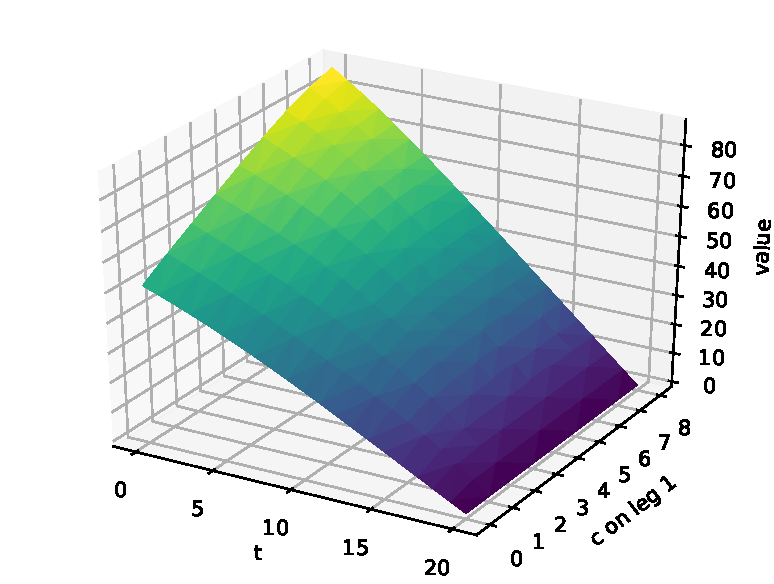
\includegraphics[width=\linewidth]{C:/Users/Stefan/LRZ Sync+Share/Masterarbeit-Klein/Code/Results/exampleStefan-True-ES-MultiLeg-190827-1516/ES-Value-c1.pdf}
		\caption{Varying capacity on leg 1.\label{fig-vF1}}
	\end{subfigure}
	\begin{subfigure}[b]{.49\linewidth}
		\centering
		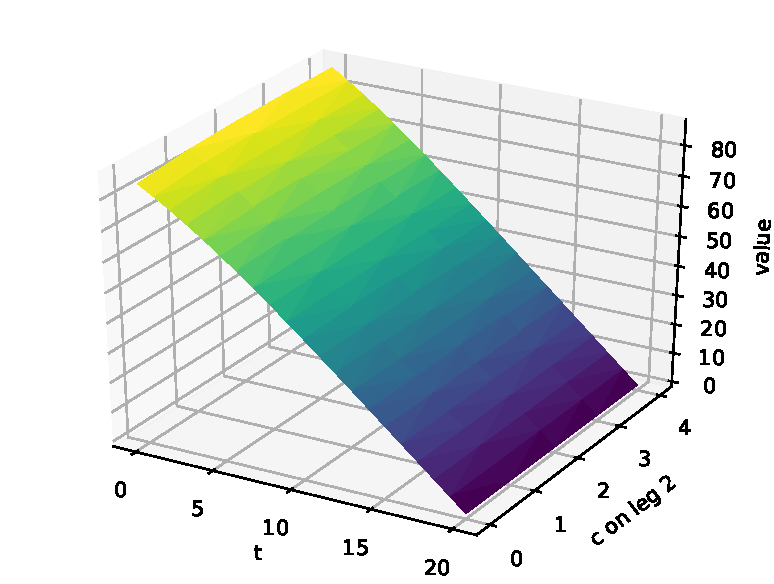
\includegraphics[width=\linewidth]{C:/Users/Stefan/LRZ Sync+Share/Masterarbeit-Klein/Code/Results/exampleStefan-True-ES-MultiLeg-190827-1516/ES-Value-c2.pdf}
		\caption{Varying capacity on leg 2.\label{fig-vF2}}
	\end{subfigure}
	\begin{subfigure}[b]{.49\linewidth}
		\centering
		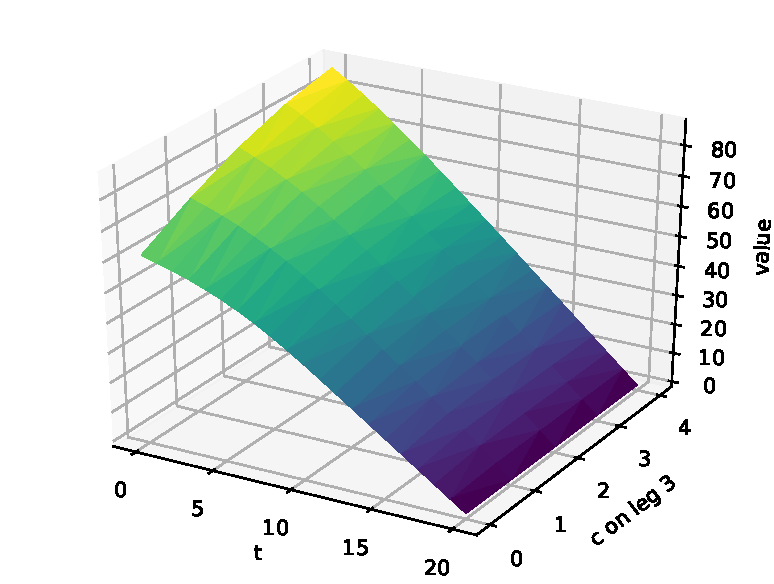
\includegraphics[width=\linewidth]{C:/Users/Stefan/LRZ Sync+Share/Masterarbeit-Klein/Code/Results/exampleStefan-True-ES-MultiLeg-190827-1516/ES-Value-c3.pdf}
		\caption{Varying capacity on leg 3.\label{fig-vF3}}
	\end{subfigure}
	\begin{subfigure}[b]{.49\linewidth}
		\centering
		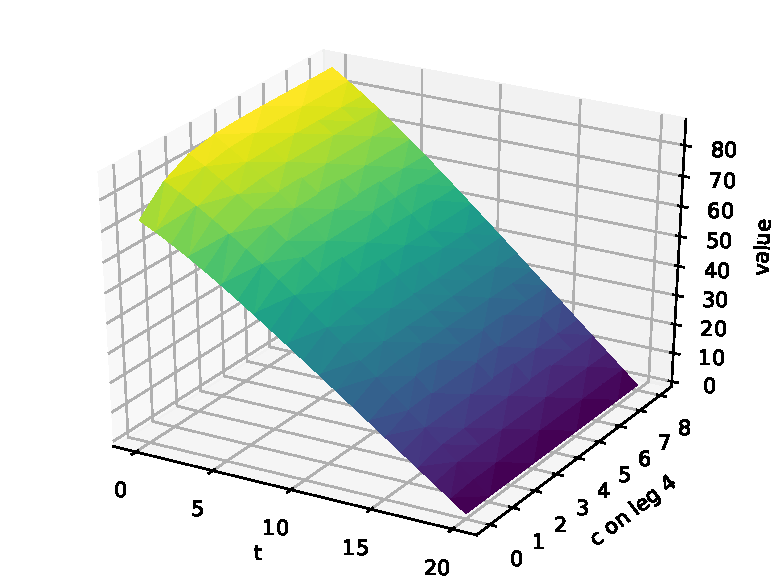
\includegraphics[width=\linewidth]{C:/Users/Stefan/LRZ Sync+Share/Masterarbeit-Klein/Code/Results/exampleStefan-True-ES-MultiLeg-190827-1516/ES-Value-c4.pdf}
		\caption{Varying capacity on leg 4.\label{fig-vF4}}
	\end{subfigure}
	\caption[Value function of working example.]{\label{fig-valueFunc}Value function of working example with time $t \in [20]$ on x-axis, capacity as stated on the y-axis (remaining capacities set to their maximal value) and the value depicted on z-axis.}
\end{figure}

\todo{Ergänze Machbarkeitsanalyse in Tabellenform (Speicherbedarf plus Rechenzeit), s. hierzu VL-Unterlagen Künstl. Intelligenz}
ES is difficult to apply in practice, mainly due to two issues as pointed out \eg in \cite{Koch.2017}. First, the decision problem inherent at each state (time period $t$ together with capacity $\boldsymbol{c}$) is an assortment optimization problem over $2^n$ possible offer sets, \ie exponential in the total number of products $n$. Already our tiny working example with $6$ products (compare \Cref{tb:AirDesc:Prod}) leads to $2^6 = 64$ offer sets.
\todo{Kann das im Cache gespeichert werden (Python und Betriebssystem)}
Second, for each time period $t$, the value function (\ref{eq:Bellman}) has to be computed for all possible combinations of capacities. This as well leads to exponential complexity, this time in the total number of resources $m$. In general, $\prod_{h \in [m]} (c^0_h+1)$ instances have to be solved\footnote{The capacity of each resources can take values in $\{0, 1, \dots, c^0_h\}$}. Already our tiny working example with $4$ resources (compare \Cref{tb:AirDesc:Res}) leads to a total of $9\cdot 5\cdot 5\cdot 9 = 2.025$ instances.


\subsection{Choice based linear programming}\label{ss:cdlp}

Because of the challenges for the exact solution as stated above, approximations are needed to solve \Cref{eq:Bellman}. A popular approach is to approximate the stochastic quantities (purchase probabilities) by deterministic values such as their expected value and to allow capacity and demand to be continuous. This approach is named \emph{Choice based linear programming} (CDLP\nomenclature{CDLP}{choice-based linear program}) and is applied by \eg \cite{GGallego.}, \cite{Liu.2008} or \cite{Bront.2009}. In the following, we first introduce the concepts underlying CDLP and its direct implementation in \cref{ss:cdlp1}. Afterwards, we present two different Column Generation techniques in \Cref{ss:cdlp2}\,.

\subsubsection{CDLP Model and direct implementation}\label{ss:cdlp1}

Taking an eagle-eye perspective, the company has to decide which sets to offer in every single time period. But as purchase probabilities don't change over time, the specific time period when to offer an individual set is indistinguishable. Thus, we can aggregate over time. We introduce a few more notation to get a hand on this. Considering one time period: As already stated in \Cref{sss:DCM}, $p_{\boldsymbol{x}}(j)$ can be interpreted as the deterministic quantity of product $j$ being sold. Let $R(\boldsymbol{x})$ represent the expected (thus deterministic) revenue given offer set $\boldsymbol{x}$, and let $\boldsymbol{Q}(\boldsymbol{x}) = (Q_1(\boldsymbol{x}), \dots, Q_m(\boldsymbol{x}))^\intercal$ denote the expected capacity being used, \ie

\begin{align}
R(\boldsymbol{x}) &= \sum_{j \in [n]} r_j p_{\boldsymbol{x}}(j)\\
Q_h(\boldsymbol{x}) &= \sum_{j \in [n]} a_{hj} p_{\boldsymbol{x}}(j) ~\forall h \in [m]
\end{align}

Note that before, we considered just one time period. Now, we aggregate over time periods and denote the total time\footnote{Total time meaning number of time periods.} for which set $\boldsymbol{x}$ is offered by $t(\boldsymbol{x})$ and the set of all possible offersets as $N = \{0,1\}^n$\,. Thus, we can formulate the choice-based linear program $V^{CDLP}(T, \boldsymbol{c})$\,.\footnote{Note that in our formulation, $p_{\boldsymbol{x}}(j)$ already includes the arrival rate $\lambda$ and thus, $\lambda$ doesn't appear directly in our formulation of CDLP in contrast to the formulation in \cite{Bront.2009}.} The optimization problem is solved by varying the decision variables $t(\boldsymbol{x})$. 

\begin{align}
V^{CDLP}(T, \boldsymbol{c}): \qquad\qquad & \max\, \sum_{\boldsymbol{x}\in N} R(\boldsymbol{x}) t(\boldsymbol{x})\label{eq:CDLP}\\
\text{s.t. } & \sum_{\boldsymbol{x}\in N} Q_h(\boldsymbol{x}) t(\boldsymbol{x}) \leq c_h ~\forall h \in [m]\label{eq:CDLP-m}\\
& \sum_{\boldsymbol{x}\in N} t(\boldsymbol{x}) \leq T\label{eq:CDLP-1}\\
& t(\boldsymbol{x}) \geq 0 ~\forall \boldsymbol{x} \in N
\end{align}

We want to mention some characteristics of this optimization problem. By allowing $t(\boldsymbol{x})$ to be continuous\footnote{E.\,g.\xspace $t(\boldsymbol{x})=1.2$ corresponds to offerset $\boldsymbol{x}$ being offered for one whole time period and $20\,\%$ of another time period.}, we arrive at a classical \emph{linear programming problem} (LP\nomenclature{LP}{linear programming problem}), for which efficient solution methods exist (such as Simplex) and are implemented (\eg in Gurobi). Even though the number of variables is exponential ($2^n$ as $N = \{0,1\}^n$), methods such as column-generation techniques can be used to solve this LP efficiently and we introduce in \Cref{ss:cdlp2}\footnote{Note that Gurobi is high-level and thus programmed in such way so that it realizes which method shall be used to solve a given LP efficiently.}. We now use concepts of duality theory to lead the way to column generation techniques.

For a start, note that the optimization problem $V^{CDLP}(T, \boldsymbol{c})$ has $m+1$ constraints - $m$ in Constraint (\ref{eq:CDLP-m}) and $1$ in Constraint (\ref{eq:CDLP-1}). By duality theory and especially Complementary Slackness, compare \eg to \cite{Domschke.2015}, at most $m+1$ basic variables will end up being non-zero. Hence, even though the number of variables being exponentially large ($2^n$), the solution will comprise at most a linear number ($m+1$) of variables, which again motivates the usage of column-generation techniques.

The dual of the CDLP is given by
\begin{align}
	VD^{CDLP}(T, \boldsymbol{c}): \qquad \min\, &\boldsymbol{\pi}^\intercal \boldsymbol{c} + \sigma T\\
	\text{s.t. } &\boldsymbol{\pi}^\intercal \boldsymbol{Q}(\boldsymbol{x}) + \sigma \geq R(\boldsymbol{x}) ~\forall \boldsymbol{x}\in N\\
	& \boldsymbol{\pi} \geq 0\\
	& \sigma \geq 0 
\end{align}
where $\boldsymbol{\pi} \in \mathbb{R}^m$ is the vector of dual variables corresponding to the resource constraints (\ref{eq:CDLP-m}) and $\sigma$ is the dual variable corresponding to the time constraint (\ref{eq:CDLP-1})\,. Again with theory of duality in mind, the optimal value of $\pi_h$ estimates the marginal value of resource $h$ and the optimal value of $\sigma$ provides a marginal value of time, \ie one additional time period would lead to an expected increase in revenue of $\sigma$ units.

In our working example, there are $256 = 2^8$ offersets and the optimal solution is presented in \Cref{txt-CDLP-Stefan}.

\begin{figure}[!ht]
	\verbatiminput{"C:/Users/Stefan/LRZ Sync+Share/Masterarbeit-Klein/Code/Results/exampleStefan-True-CDLP-190902-1649/CDLP-with-NullSet.txt"}
	\caption{Optimal solution with the null set present at start.\label{txt-CDLP-Stefan}}
\end{figure}


\subsection{Solving CDLP by Column Generation}\label{ss:cdlp2}

The huge problem size, note again the $2^n$ primal variables in \Cref{eq:CDLP} might cause problems, but can be taken care of by column generation techniques as done by \eg \cite{GGallego.}, \cite{Liu.2008} or \cite{Bront.2009}. We first sketch the algorithm, then elaborate on its complexity and finally present approaches for solving the problem.

\subsubsection{CDLP Column Generation Algorithm}

We shortly present the idea of CDLP and will elaborate in the details in the following paragraphs. The idea to handle the exponential problem size lies in starting with a small number (\eg one) of initial offer tuples and incrementally adding promising offer tuples. We start with one offer tuple $\boldsymbol{x}_1$\footnote{In alignment with \cite{Bront.2009}, this offerset comprises the first product of interest of each customer segment.}, \ie only one primal variable (instead of $N$) and solve a reduced linear program using only this column. After checking for the existence of any other offersets with positive reduced cost relative to the current dual prices of the reduced problem, we add a corresponding positive reduced cost primal variable and re-optimize the LP. If no offerset with positive reduced cost exists, the current solution of the problem is optimal.

The reduced primal CDLP problem at step \emph{k}, \ie with $k$ distinct offersets included in the set $\mathcal{N}=\{\boldsymbol{x}_1, \dots, \boldsymbol{x}_k\}$, is given by

\begin{align}
V^{CDLP-R}(T, \boldsymbol{c}): \qquad\qquad & \max \sum_{\boldsymbol{x}\in \mathcal{N}} R(\boldsymbol{x}) t(\boldsymbol{x})\label{eq:CDLPr}\\
\text{s.t. } & \sum_{\boldsymbol{x}\in \mathcal{N}} Q_h(\boldsymbol{x}) t(\boldsymbol{x}) \leq c_h ~\forall h \in [m]\\
& \sum_{\boldsymbol{x}\in \mathcal{N}} t(\boldsymbol{x}) \leq T\\
& t(\boldsymbol{x}) \geq 0 ~\forall \boldsymbol{x} \in \mathcal{N}
\end{align}

Again, with $\boldsymbol{\pi} \in \mathbb{R}^m$, resp.\xspace $\sigma \in \mathbb{R}$ denoting the dual variables of resources, resp.\xspace time, the corresponding dual problem is given by

\begin{align}
VD^{CDLP-R}(T, \boldsymbol{c}): \qquad \min\, &\boldsymbol{\pi}^\intercal \boldsymbol{c} + \sigma T\label{eq-CDLPr}\\
\text{s.t. } &\boldsymbol{\pi}^\intercal \boldsymbol{Q}(\boldsymbol{x}) + \sigma \geq R(\boldsymbol{x}) ~\forall \boldsymbol{x}\in \mathcal{N}\label{eq-CDLPr-col}\\
& \boldsymbol{\pi} \geq 0\\
& \sigma \geq 0
\end{align}

Let us analyse $V^{CDLP-R}(T, \boldsymbol{c})$ in more depth to explore the ideas behind column generation algorithms. \Cref{eq-CDLPr} shall be minimized by altering the (dual) variables $\boldsymbol{\pi}$ and $\sigma$. These variables are bounded from below by zero and have to satisfy Constraint (\ref{eq-CDLPr-col})\,. At this point, we introduce the reduced costs of an offerset $\boldsymbol{x}$ as 
$$rc(\boldsymbol{x}) \coloneqq R(\boldsymbol{x}) - \boldsymbol{\pi}^\intercal \boldsymbol{Q}(\boldsymbol{x}) - \sigma$$
and realize that Constraint (\ref{eq-CDLPr-col}) is equivalent to $rc(\boldsymbol{x}) \leq 0$, \ie all offersets in $\mathcal{N}$ are ensured to have negative reduced costs (the dual variables are chosen in such manner). Remember $N = \{0, 1\}^n$, thus we skipped all offersets $\boldsymbol{x} \in N \backslash \mathcal{N}$. If an offerset $\hat{\boldsymbol{x}}$ currently has negative reduced costs, adding $\hat{\boldsymbol{x}}$ to $\mathcal{N}$ results in one additional line of Constraint (\ref{eq-CDLPr-col}), which is inactive, \ie satisfied (we added variable $\hat{\boldsymbol{x}}$ with negative reduced costs). Thus, the objective value wouldn't change as the additional constraint doesn't put a restriction on the optimal dual variables $\boldsymbol{\pi}$ and $\sigma$. In the contrary, when considering an offerset $\check{\boldsymbol{x}}$ with positive reduced costs, adding the corresponding constraint in the dual problem results in a violation of Constraint (\ref{eq-CDLPr-col})\,. Thus, the corresponding constraint is active and $\boldsymbol{\pi}$ and $\sigma$ have to be adjusted to become admissible again. 

Having this idea in mind motivates the column generation subproblem:\footnote{Note that in comparison to \cite{Bront.2009}, the potential offersets to consider can be limited to $N \backslash \mathcal{N}$ as $\boldsymbol{\pi}$ and $\sigma$ are chosen in such manner that $rc(\boldsymbol{x}) \leq 0$ is ensured $\forall \boldsymbol{x}\in \mathcal{N}$.}

\begin{align}
	\max_{\boldsymbol{x} \in N}\, rc(\boldsymbol{x}) = \max_{\boldsymbol{x} \in N}\, \left(R(\boldsymbol{x}) - \boldsymbol{\pi}^\intercal \boldsymbol{Q}(\boldsymbol{x})\right) - \sigma \label{eq-ColGen}
\end{align}

If the optimal solution to Problem (\ref{eq-ColGen}) is positive, we augment $\mathcal{N}$ with the corresponding $\hat{\boldsymbol{x}} = \argmax_{\boldsymbol{x} \in N} rc(\boldsymbol{x})$\,. Note once again, $rc(\hat{\boldsymbol{x}}) > 0$ and thus $\hat{\boldsymbol{x}}$ is not part of the old $\mathcal{N}$\,. 

If the optimal solution to \Cref{eq-ColGen} is non-positive, the current solution is already optimal. Let's elaborate on this. $V^{CDLP}(T, \boldsymbol{c})$ differs from $V^{CDLP-R}(T, \boldsymbol{c})$ only in the considered set of offersets, all $N$ versus the reduced $\mathcal{N}$. We augmented $\mathcal{N}$ to a point, when the column generation subproblem (\ref{eq-ColGen}) results in a non-positive solution. Now, Constraint (\ref{eq-CDLPr-col}) is satisfied $\forall \boldsymbol{x} \in \mathcal{N}$ (by construction), but also $\forall \boldsymbol{x} \in N$ (compare to the optimal solution of the column generation subproblem). In summary, the optimal value of $VD^{CDLP-R}(T, \boldsymbol{c})$ equals the optimal value of $VD^{CDLP}(T, \boldsymbol{c})$. Furthermore, $VD^{CDLP}(T, \boldsymbol{c})$ equals $V^{CDLP}(T, \boldsymbol{c})$ as strong duality holds because we are dealing with a linear optimization problem and have found a feasible solution for the dual, which is a sufficient condition for strong duality as proven in Theorem $6.1.7 b)$ of \cite{Gritzmann.2013}.

Note that, up to now, we have not considered a particular customer choice model. Let us continue with introducing the MNL choice model also in the CDLP context, in order to analyse its complexity in the following. With MNL as customer choice model, \Cref{eq-ColGen}  can be expressed as (all equivalent)

\begin{align}
&\max_{\boldsymbol{x} \in \{0, 1\}^n}\left\{ \sum_{j \in [n]} r_j p_{\boldsymbol{x}}(j) - \sum_{h \in [m]} a_{hj} \pi_h p_{\boldsymbol{x}}(j) \right\} - \sigma\\
&\max_{\boldsymbol{x} \in \{0, 1\}^n}\left\{ \sum_{j \in [n]} \left(r_j  - A_j^\intercal\boldsymbol{\pi}\right) p_{\boldsymbol{x}}(j) \right\} - \sigma\\
&\max_{\boldsymbol{x} \in \{0, 1\}^n}\left\{ \sum_{l \in [L]} \lambda_l \frac{\sum_{j \in [n]} \left(r_j  - A_j^\intercal\boldsymbol{\pi}\right)u_{lj}x_j}{\sum_{j \in [n]} u_{lj}x_j + u_{l0}} \right\} - \sigma\\
&\max_{\boldsymbol{x} \in \{0, 1\}^n}\left\{ \sum_{j \in [n]} \left(r_j  - A_j^\intercal\boldsymbol{\pi}\right) x_j \left( \sum_{l \in [L]} \frac{\lambda_l u_{lj} }{\sum_{j \in [n]} u_{lj}x_j + u_{l0}} \right)\right\} - \sigma\label{eq-ColGen-sub}
\end{align}

Note that the assumptions $u_{lj} \in \mathbb{R}^+_0 ~\forall j \in [n]$, resp. $u_{l0} \in \mathbb{R}^+$ ensure the optimization problem to be well defined.

\subsubsection{Complexity of Column Generation}

As noted in \cite{Bront.2009}, \Cref{eq-ColGen-sub} is in general not separable in the variables $x_j,~j\in[n]$. Multiple customer segments (\eg $l_1$ and $l_2$) might be interested in the same product $j$ and thus, $x_j$ appears in the denominator belonging to $l_1$ and in the one belonging to $l_2$. Our column generation problem is part of the general group of \emph{hypberbolic} (or fractional) \emph{0-1 programming problems}, which were studied by \eg \cite{Hansen.1991} or \cite{Borrero.2017} and the most general version is given by

\todo{footnote to max(x) = min(-x) even if x aus 0, 1}

\begin{align}
	\max_{\boldsymbol{x} \in \{0,1\}^n} \sum_{l \in [L]} \frac{a_{l0} + \sum_{j \in [n]}a_{lj}x_j}{b_{l0} + \sum_{j \in [n]} b_{lj}x_j}~,\label{eq-hyp}
\end{align}

with no restrictions on $a_{lj}, b_{lj}$ and $x_j \in \{0, 1\} ~\forall j \in [n]$. \cite{Prokopyev.2005} have proven that \Cref{eq-hyp} is NP-hard by providing a polynomial reduction from the weighted 2SAT problem. 

\todo{ggf. Einschub von Ryzin and Liu (2004, §6.3.1) zu disjoint segments}

\todo{Give example on difficult linkage.}
\cite{Bront.2009} point out that due to the tight linkage of variables in our column generation subproblem, the general \Cref{eq-hyp} cannot be easily reduced to the specific \Cref{eq-ColGen-sub}. But they reduce the \emph{minimum vertex cover problem} to our problem \Cref{eq-ColGen-sub}. And as \cite{Garey.ca.2009} proofs the \emph{minimum vertex cover problem} to be NP-hard\footnote{Stated in [GT1] Vertex Cover under \emph{A1.1 Covering and Partitioning} on page 190 and referred to \cite{Karp.2010}, who proves NP-hardness by a transformation from 3SAT, the well established example for a problem of the NP-class.}, our column generation problem is NP-hard as well. 

\subsubsection{Approaches for solving Column Generation}

Despite the previous theoretical result, two approaches for solving column generation proofed themselves valuable in practice and are presented in the following.

\bigskip
\textbf{MIP Formulation}

We follow \cite{Bront.2009} to formulate the column generation problem \Cref{eq-ColGen} as \emph{mixed integer problem} (MIP\nomenclature{MIP}{mixed integer problem}). We face two causes of non-linearity: a fraction and a product. To eliminate the fraction, we introduce the variable
\begin{align}
	y_l = \frac{1}{\sum_{j \in [n]} u_{lj}x_j + u_{l0}}
\end{align}
and enforce this to hold via the (non-fractional) Constraint (\ref{const-frac}). By also changing the order of summation\footnote{Changing the order of summation doesn't change the summation value since the sum is finite.}, using the distributive law and ignoring the constant $\sigma$ (we check if the optimal result is $> \sigma$ in the end\todo{check if optimal column generation is greater sigma}), we rewrite the column generation problem \Cref{eq-ColGen-sub} as\footnote{Note that \cite{Bront.2009} used sloppy notation by claiming $j\in N$, as she introduced $N$ to be a constant (the total number of products). Our notation is precise.}

\begin{gather}
	\max_{\boldsymbol{x}, \boldsymbol{y}}\, \sum_{l \in [L]}\sum_{j \in [n]} (r_j - A_j^\intercal\boldsymbol{\pi}) x_j \lambda_l u_{lj} y_l\\
	\begin{align}
	\text{s.t. }y_l u_{l0} + \sum_{j \in [n]} u_{lj} x_j y_l = 1 &~\forall l \in [L]\label{const-frac} \\
	x_j \in \{0, 1\} &~\forall j \in [n]\\
	y_l \geq 0 &~\forall l \in [L]
	\end{align}
\end{gather}

To eliminate the product $x_j y_l$, we follow the concept of linearizing $x y$ with $x\in \{0, 1\}$ and $y \geq 0$ as presented by \cite{Klein.2017}. We introduce an auxiliary variable $z \geq 0$. Obviously, we want $z = 0$ if $x=0$. This leads to the constraint $z \leq x y$. And we want $z = y$ if $x=1$. This can be enforced by putting the constraints $z \leq y$\footnote{Note that this constraint is already included in the previous one $z \leq y x$, thus can be excluded here. This thought can be used to enhance \cite{Klein.2017} by combining constraints (1.20) and (1.21) to $\lambda_{ij} \leq p_j x_{ij}$. Note that constraint (1.20) does not really come from enforcing the linearization, but from the participation constraint (1.14).} and $z \geq y - M(1-x)$ with $M$ large enough.\footnote{This idea of introducing a large constant to switch off a constraint if need be is generally referred to as \emph{big M}.} Note that the other constraints are trivially fulfilled if $x=1$, resp. $x=0$. We apply these ideas and introduce the auxiliary variable $z_{lj} = x_j y_l$ with the corresponding constraints to obtain the MIP formulation

{\setlength{\abovedisplayskip}{0pt}
	\setlength{\belowdisplayskip}{0pt}
\begin{align}
		\max_{\boldsymbol{x}, \boldsymbol{y}} \sum_{l \in [L]}\sum_{j \in [n]} (r_j - A_j^\intercal\boldsymbol{\pi}) \lambda_l u_{lj} z_{lj}
\end{align}%
\begin{align}
	\text{s.t. }y_l u_{l0} + \sum_{j \in [n]} u_{lj} z_{lj} = 1 &~\forall l \in [L]\\
	y_l - z_{lj} \leq M(1-x_j) &~\forall l\in [L]\,\forall j \in [n]\label{M}\\
	z_{lj} \leq y_l x_j &~\forall l\in [L]\,\forall j \in [n]\label{z}\\
	x_j \in \{0, 1\} &~\forall j \in [n]\\
	y_l \geq 0 &~\forall l \in [L]\\
	z_{lj} \geq 0 &~\forall l\in [L]\,\forall j \in [n]
\end{align}}

\noindent with $M \geq 1/\min\{u_{l0}: l\in [L]\}$\footnote{In comparison to \cite{Bront.2009}, we adopt the minimum as not all products might be in the consideration set, thus $\underline{v}$ might be $0$. Our denominator will always be nonzero, as all $u_{l0}$ are assumed to be $>0$, and will be appropriate as potentially adding some positive $u_{lj}$ just increases the denominator, thus decreases $M$.}. $M$ is large enough, because Constraint (\ref{M}) is satisfied if activated ($x_j = 0$) as $z_{lj}$ is then forced to zero by Constraint (\ref{z}) and $y_l$ potentially set to $1/u_{l0}$ by \Cref{const-frac}. 

Having such a MIP formulation allows for the usage of standard MIP solvers like Gurobi. But as the complexity result of \cite{Bront.2009} states, the column generation problem is still NP hard. Thus, we present a polynomial time heuristic.

\bigskip
\textbf{Greedy Heuristic}\label{greedyHeuristic}

To identify the most promising offerset to add to the current set of offersets $\mathcal{N}$, we use a greedy, constructive heuristic. It was suggested by \cite{Bront.2009}, with an underlying algorithm originally proposed by \cite{Prokopyev.2005b} to solve a general fractional programming problem. We adopt notation heavily to present a  more concise and mathematical version. The algorithm makes straightforward use of the most promising offersets. Note that, via the current offersets to consider $\mathcal{N}$, we arrived at values of the dual variable $\boldsymbol{\pi}$ (and $\sigma$, but this is not needed). 

The heuristic itself is given in \Cref{alg-GreedyHeuristic}\footnote{Note that our first $j^*$, found in \Cref{alg-g-3}, is in consistence with the other $j^*$'s found in \Cref{alg-g-6}, \ie including the arrival probabilities $\lambda_l$. This is not the case in \cite{Bront.2009}, compare step 3 with step 4.a.} and explained in the following. The algorithm starts in \Cref{alg-g-1} with defining the value of an offerset candidate $X$. This really just rewrites the column generation subproblem \Cref{eq-ColGen-sub} by directly summing solely over the products in the offerset candidate instead of summing over all products and just keeping those for which $x_j=1$. \Cref{alg-g-2} initializes the set final set $S$, which will comprise the offerset in the end, and the set $S'$, which contains promising products, \ie such products with positive reduced costs. In \Cref{alg-g-3}, the most promising product $j^*$ is selected. Within the loop, sets $S$ and $S'$ are updated (\Cref{alg-g-5}) and the next suitable product $j^*$ is determined. Whenever including this product $j^*$ in the offerset $S$ makes sense, \ie raising the value of the offerset, the loop iterates again. When the value function doesn't increase further, the optimal offerset $S$ is returned. 

\begin{figure}[H]
	\hrule
	\begin{algorithmic}[1] % [1] results in line numbers
		% Großes X verwendet, um Menge zu symbolisieren
		\State $\texttt{Value}(X) \coloneqq \sum_{l=1}^{L} \lambda_l \frac{\sum_{i \in X}(r_i - A_i^\intercal\pi)u_{li}}{\sum_{i \in X}u_{li} + u_{l0}}$ \label{alg-g-1}
		\State $S\coloneqq \emptyset,\quad S' \coloneqq \left\{j \in [n] : r_j - A_j^\intercal\pi > 0\right\}$ \label{alg-g-2}
		\State $j^* \coloneqq \argmax_{j \in S'} \texttt{Value}(\{j\})$ \label{alg-g-3}
		\Repeat
		\State $S \coloneqq S \cup \{j^*\},\quad S' \coloneqq S'\backslash\{j^*\}$ \label{alg-g-5}
		\State $j^* \coloneqq \argmax_{j \in S'} \texttt{Value}(S \cup \{j\})$ \label{alg-g-6}
		\Until {$\texttt{Value}(S \cup \{j^*\}) \leq \texttt{Value}(S)$\\} \label{alg-g-7}
		\Return {$S$, \eg as offerset $\boldsymbol{x}$ given by $x_j = \mathbbm{1}_{\{j \in S\}}, ~j\in[n]$} \label{alg-g-8}
	\end{algorithmic}
	\hrule
	\captionof{algorithm}{Greedy Heuristic}\label{alg-GreedyHeuristic}
\end{figure}

This heuristic has worst-case complexity of $O (n^2 L)$ as the repeat loop might run for all $n$ products and in \Cref{alg-g-6} the calculation of the $\argmax$ of $\texttt{Value}$ is done $\abs{S'}$ times with a summation over all $L$ customer segments and the remaining, $n - \abs{S'}$ products. Note that in practice, there are much less customer segments than products, \ie $L << n$, leading to less then cubic complexity in $n$.

We want to present an adopted version\footnote{We adjust parameters $\lambda_l = 1/3$ to sum up to $1$. Note, this is necessary due to our assumption of at most one customer arriving at a given point in time. To reproduce the optimal values stated in \cite{Bront.2009}, we multiply the objective value by $3$ due to the scalability of Poisson processes as stated in .}\todo{add link to proof Poisson processes} of the example in \cite{Bront.2009} to show that \Cref{alg-GreedyHeuristic} is indeed a heuristic, \ie stops without finding the optimal solution. We also use this example as first validation of our code. Consider the column generation subproblem \Cref{eq-ColGen-sub} with $n=3, L=3$, other parameters as specified in \Cref{fig-ColGen} and $\boldsymbol{\pi} = (0, 0, 0)^\intercal$. Applying our implemented functions result in \Cref{txt-CDLP-Greedy}, which proofs that the greedy heuristic was unable to find the optimum as it stopped at the optimal value of $16.66$ instead of arriving at the truly optimal $17.83$.

\begin{figure}[H]
	\begin{subfigure}[t]{.3\linewidth}
		\centering
		\caption{Airline network.}
		\begin{tikzpicture}[
		mycircle/.style={
			circle,
			draw=black,
			fill=gray,
			fill opacity = 0.3,
			text opacity=1,
			inner sep=0pt,
			minimum size=20pt,
			font=\small},
		myarrow/.style={-Stealth},
		node distance=0.6cm and 1.2cm
		]
		\node[mycircle] (cA) {$A$};
		\node[mycircle,right=of cA] (cB) {$B$};
		
		\draw[myarrow](cA) -- node[sloped,font=\small,above] {Leg 1} (cB);
		\end{tikzpicture}
	\end{subfigure}%
	\quad
	\begin{subtable}[t]{.4\linewidth}
		\caption{Products. }
		\small
		\centering
		\begin{tabular}{yxz}
			\toprule
			\text{Product} & \text{Origin-destination} & \text{Fare}\\
			\midrule
			1 & A \rightarrow B & 100\\
			2 & A \rightarrow B & 19\\
			3 & A \rightarrow B & 19\\
			\bottomrule
		\end{tabular}
	\end{subtable}%
	\quad
	\begin{subtable}[t]{.2\linewidth}
		\caption{Resources. \label{tb:ColGen:Res}}
		\small
		\centering
		\begin{tabular}{yy}
			\toprule
			\text{Leg} & \text{Capacity}\\
			\midrule
			1 & \infty\\
			\bottomrule
		\end{tabular}
	\end{subtable}
	
	\begin{subtable}{\linewidth}
		\caption{Customers.\label{tb:ColGen:Cust}}
		\small
		\centering
		\begin{tabular}{lccccc}
			\toprule
			Seg. & $\lambda_l$ & \specialcell[b]{Consideration\\tuple} & \specialcell[b]{Preference \\vector} & \specialcell[b]{No purchase \\preference} & Description\\
			\midrule
			1 & $1/3$ & $(1, 2, 3)$ & $(1, 1, 1)$ & $1$ & Flexible, (A$\rightarrow$B)\\
			2 & $1/3$ & $(2)$ & $(1)$ & $1$ & Just $2$, (A$\rightarrow$B)\\
			3 & $1/3$ & $(3)$ & $(1)$ & $1$ & Just $3$, (A$\rightarrow$B)\\
			\bottomrule
		\end{tabular}
	\end{subtable}
	\caption[Small example for illustration of sub-optimality CDLP Greedy Heuristic.]{Small example for illustration of sub-optimality of CDLP Greedy Heuristic with $T=1$ time period.\label{fig-ColGen}}
\end{figure}

\begin{figure}[H]
	\verbatiminput{"C:/Users/Stefan/LRZ Sync+Share/Masterarbeit-Klein/Code/Results/exampleGreedy-True-CDLP-190904-1355/CDLP-exampleGreedy.txt"}
	\caption[CDLP results for small example.]{Results for small example. MIP for \enquote{CDLP with MIP formualtion} vs. GH for \enquote{CDLP with greedy heuristic}.\label{txt-CDLP-Greedy}}
\end{figure}

\vspace*{1cm}
\noindent\fbox{%
	\parbox{\textwidth}{%
		Our final implementation of the CDLP by column generation consists of: First, we use the greedy heuristic to identify a promising offerset. If this method doesn't succeed, we use the exact MIP procedure. If no new offerset is identified to enter the base, we have found the optimal solution of the CDLP.%
	}%
}
\vspace*{1cm}

Applying this version of CDLP by column generation with the greedy heuristic to our running Example, we arrive at the optimal solution as presented in \Cref{txt-CDLP-ColGen-Stefan}. Note that the same solution is found as by using CDLP in its MIP formulation, compare to \Cref{txt-CDLP-Stefan}. But the column generation version with the greedy heuristic needs just $3$ columns in comparison to $256$ used by the MIP version.

\begin{figure}[H]
	\verbatiminput{"C:/Users/Stefan/LRZ Sync+Share/Masterarbeit-Klein/Code/Results/exampleStefan-True-CDLP-190904-1432/CDLP-columnGeneration.txt"}
	\caption{Optimal solution for CDLP by column generation for working example.\label{txt-CDLP-ColGen-Stefan}}
\end{figure}


\section{Approximate Dynamic Programming}\label{s:ADP}

We now move on to a new solution approach, namely approximate dynamic programming. The method is first motivated and put in context of the thesis. Second, a short classification of different methods belonging to this class is presented, before the method applied in our setting is discussed in detail.

ADP builds upon \Cref{eq:DP-optOffer}. The real challenge is to determine the opportunity costs per product $j$, \ie $\Delta_j V(t+1, \boldsymbol{c})$. ADP approximates these opportunity costs additively using bid prices for the resources $h$, $\pi_h(t, c_h)$, if those are needed to produce product $j$, \ie $\Delta_j V(t+1, \boldsymbol{c}) = \sum_{h \in [m]} a_{hj}\pi_{h}(t+1, c_h)$. Thus, the policy is given as the solution of

\begin{align}
^\pi \boldsymbol{x}^t = \argmax_{\boldsymbol{x}^t \in \{0,1\}^n}\left\{ \sum_{j \in [n]} p_j(\boldsymbol{x}^t) \left( r_j - \sum_{h \in [m]} a_{hj}\pi_{h}(t+1, c_h) \right) \right\}~,\label{eq:ADP-online}
\end{align}

and is therefore completely described by the bid prices $\pi_h(t, c_h) ~\forall t \in [T]$. Note that $\boldsymbol{x}^t$ represents the set offered during time period $t$, \ie the decision is made at time point $t-1$. $\Delta_j V(t+1, \boldsymbol{c})$ represents the difference in revenue to go when looking at selling product $j$ and considering time periods $t+1, \dots, T$ and capacities $\boldsymbol{c}$. Note that when considering the very last time period $T$, opportunity costs $\Delta_j V(t+1, \boldsymbol{c})$ are zero $\forall j \in [n], \forall \boldsymbol{c} \geq 0$.

We now present a brief overview how to classify simulation based ADP methods, which the textbooks \cite{Bertsekas.2005} and \cite{Powell.2011} cover in more detail. The methods are named \emph{approximate}, as they are based on approximating the value function. Various sample paths are generated and used in basically two different manners to iteratively improve the approximation of the value function: either by \emph{approximate value iteration} (AVI\nomenclature{AVI}{approximate value iteration}) or by \emph{approximate policy iteration} (API). Each iteration of AVI comprises a single sample path. It evaluates the current policy on this particular sample path and updates parameters for the value function approximation after each period of the sample path. In contrary, each iteration of API  comprises multiple sample paths. It evaluates the current policy on a set of sample paths and uses the combined information to update and improve the value function approximation (and thus the policy). Thus, one iteration of API is certainly costlier and usually API requires less iterations to obtain good policies. One obvious prerequisite for this is a large enough set of sample paths. We refer to \cite{Powell.2011} for more details.

A suitable method to be used for our setting was proposed by \cite{Koch.2017} and belongs to the class of simulation based ADP. More precisely, it comprises a value function approximation algorithm and uses policy iteration. It approximates the value function $V(t, \boldsymbol{c})$ by computationally simple functions (linear or piecewise linear), makes use of an offline phase to determine bid prices $\pi_h(t, c_h) ~\forall t \in [T]$ and applies \Cref{eq:ADP-online} in an online phase to compute the offerset.

\subsection{Approximate Policy Iteration}

Approximate Policy Iteration is used in the offline phase and aims at determining bid prices for each time period $\pi_h(t, c_h) ~\forall t \in [T]$, which fully determine the policy used in the online phase. The complete algorithm is given by \Cref{alg-API} and comprises several steps. We first give an overview of the concept and then explain the details step by step.

\subsubsection{API value function approximation}

We will introduce the concept of the method in the following and created \Cref{tb-api-param} for reference, as there are quite some variables involved in API.

% https://tex.stackexchange.com/questions/111110/get-a-table-and-figure-on-the-same-page-with-captions-labels
\noindent\begin{minipage}{\linewidth}
	{\small
	\begin{tabular}{lll}
		\toprule
		Symbol & Domain & Meaning\\
		\midrule
		$\theta_t$ & $\mathbb{R}$ & optimization variable (offset) for time period $t$\\
		$\Theta$ & $\mathbb{R}^\intercal$ & optimization variable comprising all $\theta_t$\\
		$\boldsymbol{\pi}_t$ & $\mathbb{R}^m$ & optimization variable (bid price for each resource) for time period $t$\\
		$\boldsymbol{\Pi}$ & $\mathbb{R}^{m \times T }$ & optimization variable (bid price for each resource) comprising all $\boldsymbol{\pi}_t$\\
		$\hat{V}^i_t $ & $\mathbb{R}$ & sample revenue to go for sample $i$ starting at and including period $t$\\
		$\hat{V}$ &  $\mathbb{R}^{T \times I}$ &all sample revenues to go comprising all $\hat{V}^i_t $ \\
		$\boldsymbol{\hat{C}}^i_{t-1}$ & $\mathbb{R}^m$ & available capacities for resources for sample $i$ at end of period $t-1$\\
		$\boldsymbol{\hat{C}}$ & $\mathbb{R}^{m \times T \times I}$ & all available capacities comprising all $\boldsymbol{\hat{C}}^i_{t-1}$\\
		$r_t$ & $\mathbb{R}$ & sample revenue generated during time period $t$\\
		$\boldsymbol{c}$ & $\mathbb{N}^m$ & available capacities for each resource at current time period\\
		$\boldsymbol{c}^0$ & $\mathbb{N}^m$ & starting capacities\\
		$\boldsymbol{x}$ & $\{0,1\}^n$ & offerset at current time period\\
		$\epsilon_t$ & $[0,1]$ & epsilon used at time period $t$\\
		\bottomrule
	\end{tabular}
	}
	\captionof{table}{API overview of parameters.\label{tb-api-param}}
	
	\vspace*{0.5cm}
	\hrule
	\begin{algorithmic}[1]
		\State Set $\theta_t = 0$ and $\boldsymbol{\pi}_t = \boldsymbol{0} ~\forall t \in [T]$ \label{alg-API1}
		\For{\texttt{k = 1 to K}} \label{alg-API-Piter1}
		\State Set $\hat{V}_t^i = 0$ and $\boldsymbol{\hat{C}}_{t-1}^i = 0 ~\forall t \in [T], \forall i \in [I] $ \label{alg-API3}
		\For{\texttt{i = 1 to I}}\label{alg-API-Peval1}
		\State Set $\hat{r}_t = 0$ and $\boldsymbol{\hat{c}}_{t-1} = 0 ~\forall t \in [T]$ \label{alg-API5}
		\State Initialize $\boldsymbol{c} = \boldsymbol{c}^0$\label{alg-API6}
		\For{\texttt{t = 1 to T}}
		\State $\boldsymbol{\hat{c}}_{t-1} \coloneqq \boldsymbol{c}$\label{alg-API8}
		\State Get $\boldsymbol{\pi}(t, \boldsymbol{c})$ \label{alg-API-calcPi}
		\State Compute $\boldsymbol{x} = \texttt{determineOfferset}(\boldsymbol{\pi}(t, \boldsymbol{c}), \epsilon_t)$ \label{alg-API10}
		\State Simulate a sales event $j' \in \{0, 1, \dots, n\}$\label{alg-API11}
		\If{$j' \in \{ 1, \dots, n\}$}
		\State $\hat{r}_t = r_{j'}$ and $\boldsymbol{c} = \boldsymbol{c} - \boldsymbol{a}_{j'}$\label{alg-API13}
		\EndIf
		\EndFor
		\State Compute $\hat{V}_t^i = \sum_{\tau = t}^{T}\hat{r}_t ~\forall t \in [T]$\label{alg-API14}
		\State Assign $\boldsymbol{\hat{C}}_{t-1}^i = \boldsymbol{\hat{c}}_{t-1} ~\forall t \in [T]$ \label{alg-API15} 
		\EndFor
		\State $\left(\Theta, \boldsymbol{\Pi} \right) = \texttt{updateParameters}(\hat{V}, \boldsymbol{\hat{C}}, \Theta, \boldsymbol{\Pi}, k)$ \label{alg-API-updateParam}
		\EndFor
		\State \Return {$\left(\Theta, \boldsymbol{\Pi} \right)$}
	\end{algorithmic}
	\hrule
	\captionof{algorithm}{Approximate policy iteration. Note that $t$ represents a time period and therefore takes values in $[T]$. As at time period $t$, there is $c_{t-1}$ capacity available, we use a different index for capacity.}\label{alg-API}
\end{minipage}

API aims at approximating the value function for each state. A state is characterized by current time period $t$ and vector of current capacities $\boldsymbol{c}$. Therefore, a natural choice is to use a linear function as given by

\begin{align}
&V_{t,\boldsymbol{c}}(\theta_t, \boldsymbol{\pi}_t) \coloneqq \theta_t + \sum_{h \in [m]} \pi_{th} c_h\\
&\text{with}\nonumber\\
&~~~\theta_t \geq 0\label{eq-api-theta}\\
&\max_{j=1, \dots, n} r_j \geq \pi_{th} \geq 0\label{eq-api-pi}
\end{align}

\todo{graph: Add graph, why the two other constraints are necessary}
and $\theta_{T+1} = 0$ as well as $\pi_{T+1, h} = 0 ~\forall h\in[m]$ assumed implicitly, thus leading to $V(T+1, \boldsymbol{c}) = 0$ if $\boldsymbol{c} \geq \boldsymbol{0}$. Note that we follow \cite{Koch.2017} and include expert knowledge on the problem. The non-negativity constraints in \Cref{eq-api-theta} and \Cref{eq-api-pi} ensure that the optimal value is non-negative and increasing in capacity. The upper bound in \Cref{eq-api-pi} is also reasonable as one additional capacity should increase the optimal value less than the amount of revenue generated by selling the most expensive product. This directly leads us to the interpretation of the variables. $\theta_t$ represents the constant offset. $\pi_{th}$ can be directly interpreted as bid prices of the resources, and therefore be used in \Cref{eq:ADP-online}:  $\pi_h(t, c_h) = \pi_{th}$. Note that in this setting, the bid price is independent of the current level of capacity.\footnote{In comparison of a linear with a piecewise linear approach.}

\subsubsection{API overview}

Let us now discuss the algorithm in depth.\footnote{We strictly use our notion of time periods in this thesis. Note that there is a one-to-one correspondence of \enquote{action happening during time period $t$ with $t\in[T]$} and \enquote{action happening at time point $t$ with $t\in \{0, \dots, T-1\}$}. The latter is more convenient to use in the Python implementation as Python indexing starts at $0$.} For the first policy iteration, \Cref{alg-API1} sets all optimization variables to zero which results in the greedy policy of offering the set resulting in the highest expected revenue (no consideration of costs) in each time period.

Then, a total of $K$ policy iterations follow.\footnote{Note that this direct approach is used in \cite{Koch.2017}. While a suitable $K$ was presumably found looking at convergence rates and then fixed, I would encourage practitioners to directly apply a convergence criterion for termination of policy iteration. Note that policy iteration is proven to converge if a discounting factor of later revenues is included. Compare \citeauthor{Bertsekas.2005}(\citeyear{Bertsekas.2005}; Proposition 1.3.6 on p. 48).} In each policy iteration $k$, the current policy is evaluated first. To do so, we use the current policy to evaluate $I$ random sample paths. \Cref{alg-API3} sets up the dataset for revenues to go $\hat{V}_t^i$ and remaining capacities $\boldsymbol{\hat{C}}_{t-1}^i$ for all time periods $t \in [T]$ and sample paths $i \in [I]$. 

For each sample path $i$, a storage unit for revenue $\hat{r}_t$ is created for all time periods $t \in [T]$ and all capacities $\boldsymbol{\hat{c}}_{t-1}$ (\Cref{alg-API5}). Note, that we use a different index for capacities to account for the fact that for the remaining revenues to go starting from and including time period $t$, we have capacities $\boldsymbol{c}_{t-1}$ available (those being left over from time period $t-1$.). Furthermore, the capacity is set to the initial capacity in \Cref{alg-API6}.

For each time period, the available capacity $\boldsymbol{\hat{c}}_{t-1}$ (left over at end of previous time period) is stored in \Cref{alg-API8}, the current bid prices are calculated in \Cref{alg-API9} and used to determine the offerset $\boldsymbol{x}$ in \Cref{alg-API10}. More details on the determination of the offerset can be found in \Cref{sec-determineOfferset}. With this information, a sales event $j'$ is simulated and in case a product has been sold ($j' \in [I]$), the revenue is stored and capacity adjusted accordingly. Note, the revenue thus belongs to time period $t$ and capacity will affect time period $t+1$ (\Cref{alg-API11} to \Cref{alg-API13}).

After simulating one sample path, the value function for this sample path $\hat{V}_t$ is evaluated for all time periods $t\in[T]$ in \Cref{alg-API14}, and so are the capacities in \Cref{alg-API15}.

Finally, \Cref{alg-API-updateParam} comprises the policy improvement step and uses all the information of the current policy iteration to update the optimization variables $\theta_t, \boldsymbol{\pi}_t ~\forall t$. Before expanding on how this update is executed, we want to fill the gap on how the offerset is determined in \Cref{alg-API10}.

\subsubsection{API determination of offersets}\label{sec-determineOfferset}

Our goal is to efficiently determine a reasonable set of products to offer. Thus, we use a heuristic and reduce the amount of products to consider as fast as possible. The following algorithm is based on the ideas of the greedy, largest marginal benefit heuristic for the column generation subproblem outlined in \cite{Bront.2009} and presented above in \Cref{alg-GreedyHeuristic}.

%todo expand on exploration vs exploitation dilemma
The function $\texttt{determineOfferset}(\boldsymbol{\pi}, \epsilon)$ calculates the set of products to offer depending on the current bid prices $\boldsymbol{\pi}$ via the greedy algorithm pointed out in \cite{Bront.2009}. As we put ourselves into a policy improvement setting and started out with the greedy strategy, the whole procedure tends to find solely other policies rather closeby, \ie also greedy. Thus, we would leave out a big portion of the whole solution space (for each time period and each combination of capacities any subset of the $n$ products can be offered). This is the famous \emph{exploration vs. exploitation dilemma}. Exploitation: The current solution was found and improved already and should be exploited even further (comparable to incremental innovation). Exploration: But also other, yet to be seen parts of the solution space should be explored (comparable to disruptive innovation). To account for this dilemma, we follow \cite{Koch.2017} and use an \emph{epsilon-greedy strategy}. With a probability of $\epsilon/2$ either no product is offered at all or all products with positive contribution $r_j - \sum_{h \in [m]} a_{hj} \cdot \pi_h$ are offered. With a probability of $1-\epsilon$, the set determined by \Cref{alg-GreedyHeuristic} is offered.

Note that in the very first iteration, we do not have appropriate values for $\boldsymbol{\pi}$ and $\theta$. Thus, we decided to set them to zero at start, corresponding to \enquote{no opportunity costs of resources}.


\subsubsection{API update of parameters}\label{sec-updateParameter}

With the information of the $I$ sample paths, all optimization variables $\left(\Theta, \boldsymbol{\Pi} \right)$ are updated. Note that the old parameters are used as starting values and the current policy iteration $k$ is also passed to potentially take care of exponential smoothing. Thus, we have $(1+h)*T$ parameters ($\theta_t$ and $\boldsymbol{\pi}_t ~\forall t \in [T]$) and $TI$ data points, where each data point comprises the value of the value function as $y$-value and the current assignment of $t$ and $\boldsymbol{\pi}_t$ as $x$-values. 

The function $\texttt{updateParameters}(\hat{V}, \boldsymbol{\hat{C}}, \Theta, \boldsymbol{\Pi}, k)$ comprises the following least squares optimization problem, which optimizes all optimization variables, $(\theta_t, \boldsymbol{\pi}_t)_t$ with $t \in [T]$ at the same time and the optimal values $(\Theta^{update}, \boldsymbol{\Pi}^{update})$ are obtained.

\begin{alignat}{2}
& \text{min} \sum_{i=1}^{I}\sum_{t=1}^{T} \left( \hat{V}_t^i - V_{t\boldsymbol{c}_t^i}(\theta_t, \boldsymbol{\pi}_t) \right)^2 &&\label{opt-updateParam-beginning} \\
& \text{s.t. } && \\
& ~~\theta_t \geq 0 && \forall t \in [T]\\
& \max_{j \in [n]} r_j \geq \pi_{th} \geq 0 && \forall t \in [T], \forall h \in [m]\\
& ~~\theta_t \geq \theta_{t+1} && \forall t \in \{1, \dots, T-1\}\\
& ~~\pi_{th} \geq \pi_{t+1,h} && \forall t \in \{1, \dots, T-1\}\label{opt-updateParam-end}
\end{alignat}

The old values $\theta_t^k$ and $\boldsymbol{\pi}_t^k$ are used to determine the optimal parameter $\theta_t^{update}$ and $\boldsymbol{\pi}_t^{update}$.

There exist multiple on possibilities on which values shall be used as new optimization variables. One approach might be to just use the optimal values:
\begin{align}
\theta_t^{k+1} &= \theta_t^{update}\label{dir-1}\\
\boldsymbol{\pi}_t^{k+1} &= \boldsymbol{\pi}_t^{update}\label{dir-2}
\end{align}

Another approach is to use exponential smoothing, which assigns quite some value to the previous iterations and updates the optimization variables less and less, \ie its weights decrease with an increasing number of policy iterations $k$. Here, for the next iteration $k+1$ the values of optimization variables are calculated via:
\begin{align}
\theta_t^{k+1} &= \left(1- \frac{1}{k} \right)	\theta_t^k + \frac{1}{k} \theta_t^{update}\label{expSM-1}\\
\boldsymbol{\pi}_t^{k+1} &= \left(1- \frac{1}{k} \right)	\boldsymbol{\pi}_t^k + \frac{1}{k} \boldsymbol{\pi}_t^{update}\label{expSM-2}
\end{align}

One can also apply the first technique (use the updates directly) during the policy iteration and finally report an average over all parameter values at the very end. Note that \Cref{l-expSmooth} presents the circumstances and mathematical proof on when this procedure becomes equivalent to exponential smoothing as introduced above.
\begin{align}
\theta_t^{K+1} &= \frac{1}{K}\sum_{k=1}^{K}\theta_t^k\\
\boldsymbol{\pi}_t^{K+1} &= \frac{1}{K}\sum_{k=1}^{K}\boldsymbol{\pi}_t^k
\end{align}


\subsection{Running Example}


We evaluate different combinations of parameters and go with the same as \cite{Koch.2017}, \ie $K = 60$ policy iterations, $I = 800$ sample paths and a parameter for the epsilon-greedy strategy monotonously decreasing with the number of policy iteration $k$:

\begin{align}
\epsilon_k = 
\begin{cases}
0.05, ~ &k=1, \dots, 10\\
0.01, ~ &k=11, \dots, 20\\
0, & \text{otherwise}
\end{cases}
\end{align}

We prepare $I \times T$ random numbers for the customer streams, the sales stream and the epsilon criterion. Note that these numbers are random, but remain the same over the $K$ policy iterations. \Cref{fig-adp-epsilon} shows the distribution of a uniform random variable in the whole $I \times T$ setting. It can be clearly seen that the underlying random variable indeed follows a uniform $U(0,1)$ distribution and can thus be used for applying the epsilon-greedy strategy with thresholds as specified above. \Cref{fig-adp-customer} presents the boxplots of arriving customers. For each of the $I$ iterations, the number of arriving customers in the event horizon ($t \in [T]$) was reported and then depicted. The means can be seen to be in line with the model specification (\eg customer $1$ has arrival probability of $0.3$) and the standard deviation is fine. Thus, our exemplary data represents our model specification and we can apply approximate dynamic programming.

\begin{figure}[H]
	\begin{minipage}[t][7cm][t]{.5\textwidth}
		\centering
		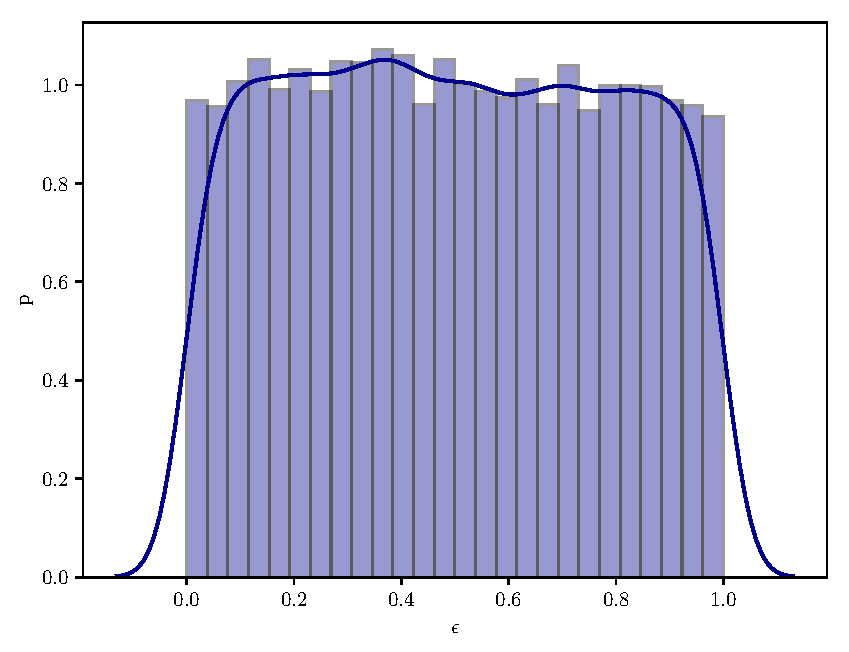
\includegraphics[height=6cm]{C:/Users/Stefan/LRZ Sync+Share/Masterarbeit-Klein/Code/Results/exampleStefan-True-APILinearMultiLeg-190918-1053/epsilon2.pdf}
%		\vfill
		\captionof{figure}{\label{fig-adp-epsilon}Distribution of epsilon values.}
	\end{minipage}%
	\begin{minipage}[t][7cm][t]{.5\textwidth}
		\centering
		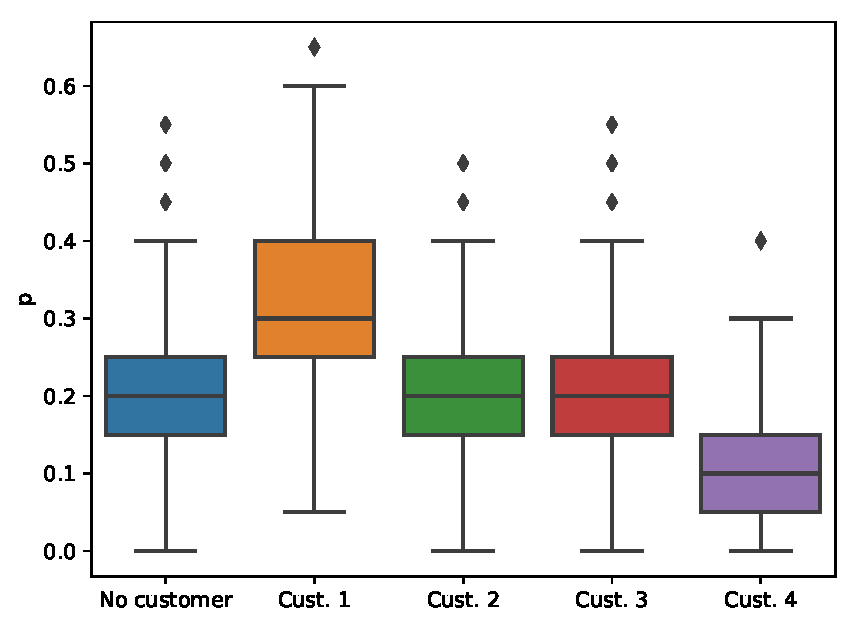
\includegraphics[height=6cm]{C:/Users/Stefan/LRZ Sync+Share/Masterarbeit-Klein/Code/Results/exampleStefan-True-APILinearMultiLeg-190918-1053/customer.pdf}
%		\vfill
		\captionof{figure}{\label{fig-adp-customer}Boxplot of customers in training.}
	\end{minipage}
\end{figure}

The evolution of the average realized value\footnote{Realized value refers to value realized over the time horizon, \ie total revenue generated due to selling of products in time periods $t\in [T]$.} over the $I$ iterations in each of the $k \in \{1, \dots, 60\}$ policy iterations is depicted in \Cref{fig-adp-valueFunc}. It can be seen, that the initial simplification of having opportunity costs of zero ($k=1$), results in a pretty high overall result. This is due to the short time frame ($20$ time periods) in combination with plenty of available resources ($24 = 8+4+4+8$), so it seems reasonable to offer as many products as possible because leftovers are worthless. Roughly $15$ policy iterations are needed before API comes back to a close to optimal average value at start. After some jumps of varying height, it is interesting that API starts in $k=53$ to oscillate between the optimal values $59.265$ and $69.9425$. This leads to the conclusion, that no stable solution can be found. This behaviour is most probably caused by the specific interaction of which customer comes when leading to varying capacities present at certain time steps, thus to different sets to be offered and ultimately purchased.

\begin{figure}[H]
	\centering
	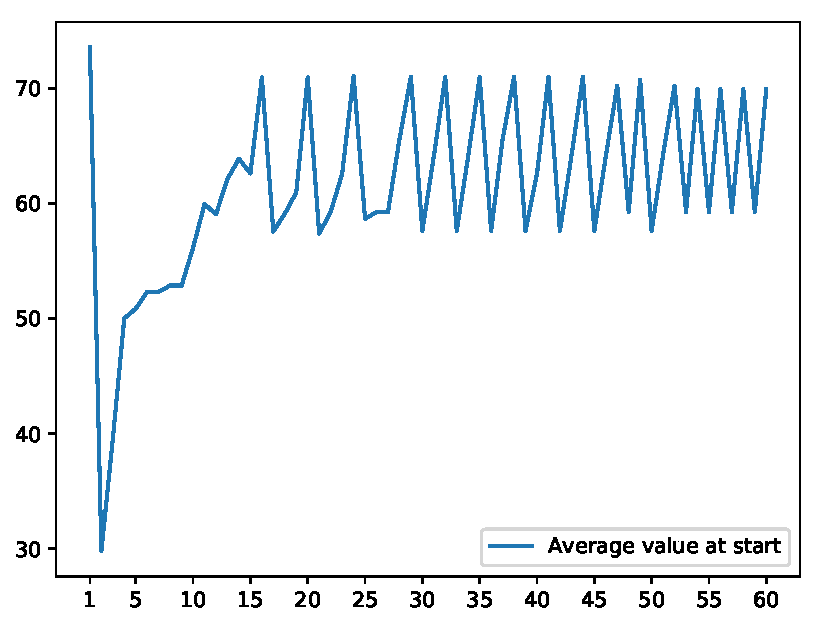
\includegraphics[width=.7\linewidth]{C:/Users/Stefan/LRZ Sync+Share/Masterarbeit-Klein/Code/Results/exampleStefan-True-APILinearMultiLeg-190918-1053/plotValue.pdf}
	\caption[Average value at start for the evolution via $K=60$ policy iterations.]{\label{fig-adp-valueFunc}Average value at start (y-axis) for the evolution via $K=60$ policy iterations (x-axis).}
\end{figure}

That some resources are still left over after the time horizon can be seen in \Cref{fig-adp-capacities}. The left graph depicts the remaining capacities after the selling horizon for each resource for the first $10$ policy iterations (aggregated over all $I=800$ sample paths). Remember that we start with $8$ units of capacity for resources $1$ and $4$, and $4$ units of capacity for resources $2$ and $3$. During the first iterations, resource $1$ is used more often then resource $4$, but still remains left over with quite some amount. This changes towards the latter iterations (right graph), when we see again the alternating behaviour and much less capacity of resource $1$ remaining.

\begin{figure}[H]
	\begin{subfigure}[t]{.5\textwidth}
		\centering
		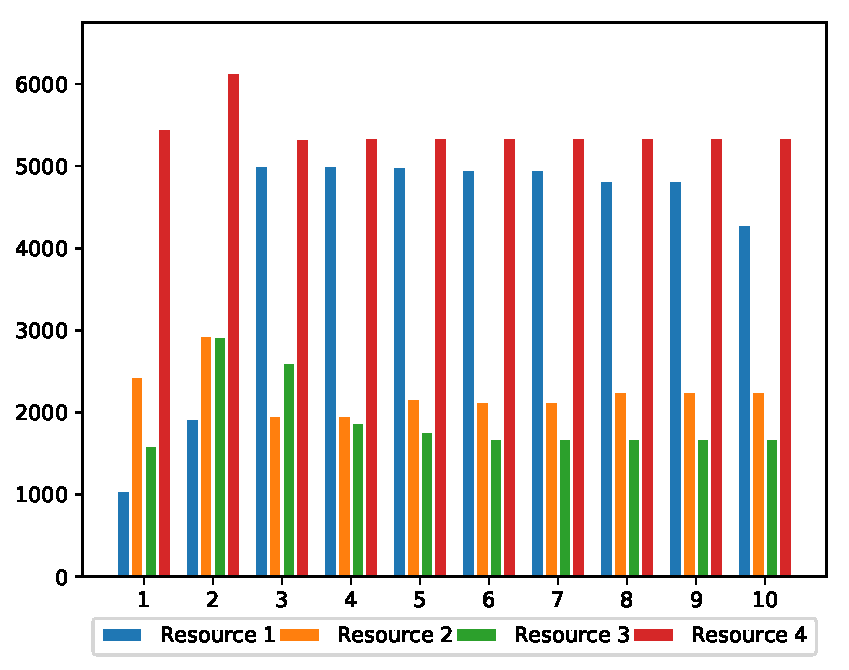
\includegraphics[width=\linewidth]{C:/Users/Stefan/LRZ Sync+Share/Masterarbeit-Klein/Code/Results/exampleStefan-True-APILinearMultiLeg-190918-1053/remainingCapacity0.pdf}
		\caption{\label{fig-adp-capacities0}$K=\{1, \dots, 10\}$}
	\end{subfigure}%
	\begin{subfigure}[t]{.5\textwidth}
		\centering
		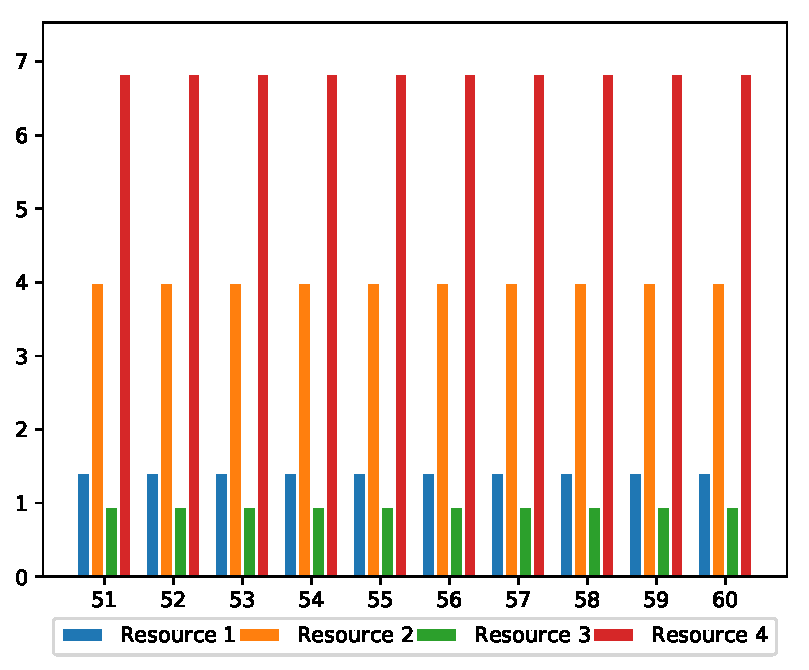
\includegraphics[width=\linewidth]{C:/Users/Stefan/LRZ Sync+Share/Masterarbeit-Klein/Code/Results/exampleStefan-True-APILinearMultiLeg-190918-1053/remainingCapacity50.pdf}
		\caption{\label{fig-adp-capacities50}$K=\{51, \dots, 60\}$}
	\end{subfigure}
	\caption[Remaining capacities via several policy iterations.]{\label{fig-adp-capacities} Remaining capacities via several policy iterations (x-axis).}
\end{figure}

This last observation goes along with the hypothesis of the oscillating solution and can also be verified by looking at \Cref{fig-adp-products}, which depicts the purchased products. \Cref{fig-adp-products1} includes the \enquote{no-purchases} explicitly, while \Cref{fig-adp-products2} depicts the purchased products stacked over each other, leading the total height of each cumulated bar to represent the total amount of purchased products. Note that summing up all purchase actions (including \enquote{no-purchase}), leads to a total of $16,000 (= 20 \times 800 = T \times I)$ in each polity iteration $k$. In combination with the value plot (\Cref{fig-adp-valueFunc}), we see that API is well suited for our problem. After the first iteration, which is needed to set up the parameters, product $2$ is sold very often. But as this is the cheapest product, even though a lot of products are sold, the average value generated is very low ($29.795$). This error is recognized immediately by API and to purely offer product $2$ is never done again as can be seen in \Cref{tb-adp-offersets}. The policy is changed and the pretty expensive product $6$ is offered most often and therefore also purchased most often ($1,281$ times, while the second most often purchased product $5$ is purchased $1,116$ times). This iteration, less products then in the previous iteration are sold, but a higher value is achieved. In the following iterations, the amount of purchased products increases more and more until a peak in iteration $16$. The,n the alternating behaviour begins. All this is also seen in the offered products as presented in \Cref{tb-adp-offersets}. Here we clearly see that the end of our optimization is reached as we oscillate back and forth from iteration $53$ onwards. The algorithm is trapped in a (stable) circle.\footnote{As exponential smoothing is closely related to an average over all policy iterations, or at least leads to the optimal values changing less and less, the value function should converge to a unique solution eventually.}\todo{Code laufen lassen, um $k$ herauszufinden}

\begin{figure}[H]
	\begin{subfigure}[t]{.5\textwidth}
		\centering	
		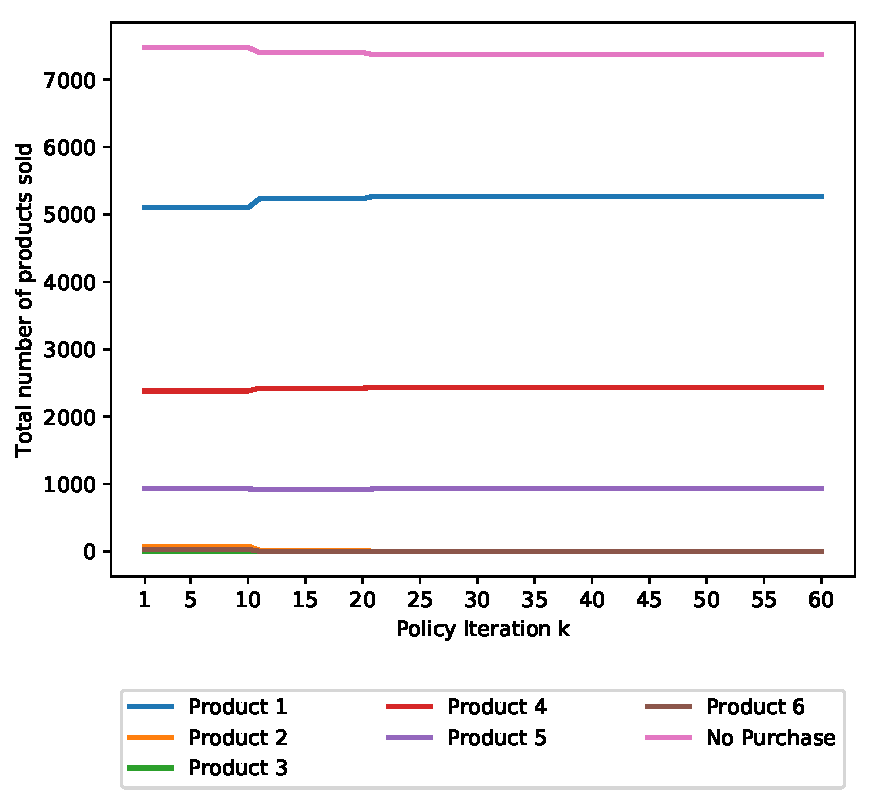
\includegraphics[width=\linewidth]{C:/Users/Stefan/LRZ Sync+Share/Masterarbeit-Klein/Code/Results/exampleStefan-True-APILinearMultiLeg-190918-1053/plotProducts1.pdf}
		\caption{\label{fig-adp-products1} With no-purchases.}
	\end{subfigure}%
	\begin{subfigure}[t]{.5\textwidth}
		\centering
		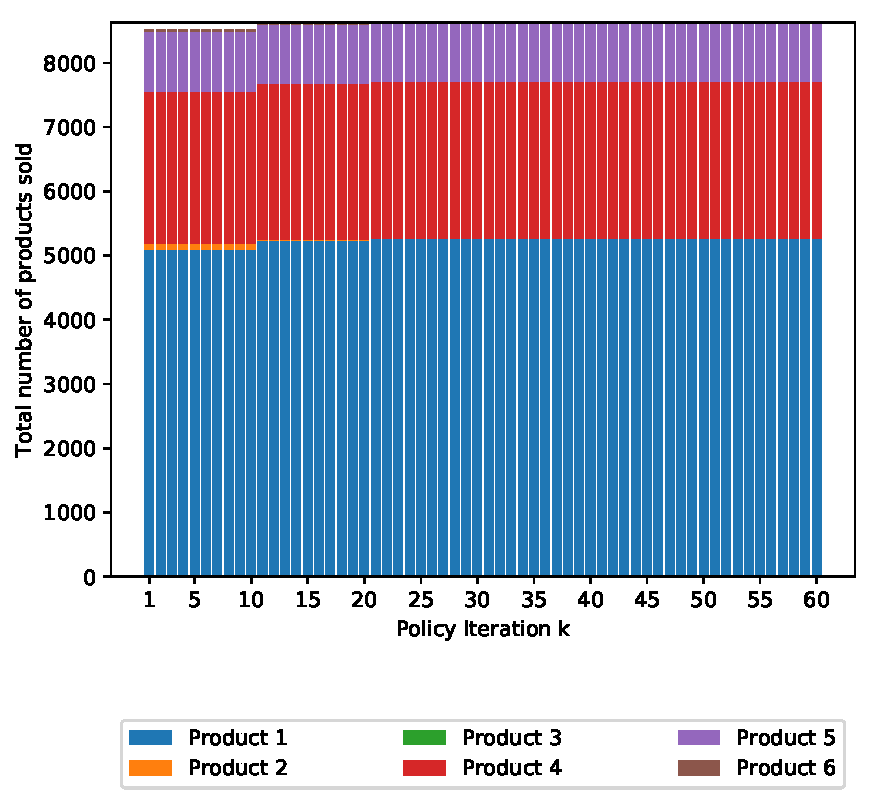
\includegraphics[width=\linewidth]{C:/Users/Stefan/LRZ Sync+Share/Masterarbeit-Klein/Code/Results/exampleStefan-True-APILinearMultiLeg-190918-1053/plotProducts2.pdf}
		\caption{\label{fig-adp-products2} Solely products.}
	\end{subfigure}
	\caption[Evolution of purchased products via $K=60$ policy iterations.]{\label{fig-adp-products}Evolution of purchased products (y-axis) via $K=60$ iterations (x-axis).}
\end{figure}

\begin{table}
	\footnotesize
	\resizebox{\linewidth}{!}{
	\input{"C:/Users/Stefan/LRZ Sync+Share/Masterarbeit-Klein/Code/Results/exampleStefan-True-APILinearMultiLeg-190918-1053/offersetsOffered.txt"}
	}
	\caption{\label{tb-adp-offersets}Sets offered via $K=60$ policy iterations in the working example.}
\end{table}

Let us explore the resulting optimal values and offer sets in a bit more detail using two more graphs. \Cref{fig-adp-pi} presents the optimal values of $\pi_{th}$ for every time period $t$ and resource $h$. Note that the optimal values are barely changing from the second-last iteration (\Cref{fig-adp-pi59}) to the last iteration (\Cref{fig-adp-pi60}). In both iterations resource $4$ has basically no opportunity costs, which is in line with the low demand for this product. The values for resources $1$ and $2$ are changing slightly, which raises the questions whether this small change even matters. Looking at \Cref{fig-adp-offersets}, it does. This figure presents the optimal offersets to be offered at any time (x-axis) and any combination of resource capacities (y-axis) in a separate colour. By \enquote{combination of resource capacities}, I refer to the following: As the vector of starting capacities for resources is given by $(8, 4, 4, 8)$ and the least amount of capacity is zero, there are a total of $9 \cdot 5\cdot 5 \cdot 9 = 2025$ combinations possible. Note however, API with linear value function approximation abstracts from these combinations, as it is not aware of the amount of available capacity. For the resulting offersets, we see that in both iteration steps, first $\{3, 5\}$ is presented to the customer and in the last time periods, $\{1, 3,4,5,6\}$ is offered. But in the in-between, at the second-last iteration, $\{1,3,5\}$ is offered just in period $3$, while for the last iteration, the transition comes via two different sets and takes longer. This figure also refers back to the identification of product $2$ of not worth offering, as explained above.


\begin{figure}[H]
	\begin{subfigure}[t]{.5\textwidth}
		\centering	
		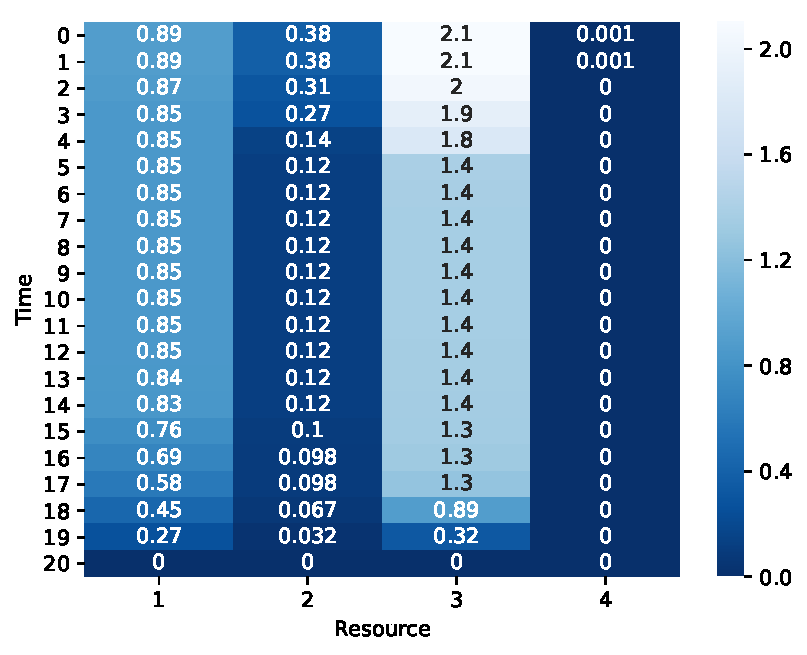
\includegraphics[width=\linewidth]{C:/Users/Stefan/LRZ Sync+Share/Masterarbeit-Klein/Code/Results/exampleStefan-True-APILinearMultiLeg-190918-1053/pi59.pdf}
		\caption{\label{fig-adp-pi59} $k=59$}
	\end{subfigure}%
	\begin{subfigure}[t]{.5\textwidth}
		\centering
		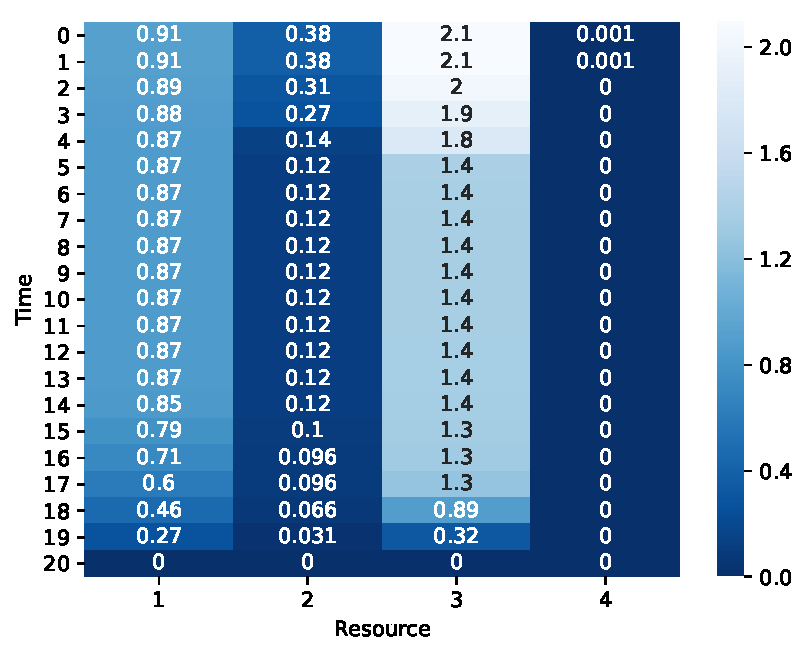
\includegraphics[width=\linewidth]{C:/Users/Stefan/LRZ Sync+Share/Masterarbeit-Klein/Code/Results/exampleStefan-True-APILinearMultiLeg-190918-1053/pi60.pdf}
		\caption{\label{fig-adp-pi60} $k=60$}
	\end{subfigure}
	\caption{\label{fig-adp-pi}Heatmap of optimal values for $\pi_{th}$ for the two final policy iterations.}
\end{figure}

\begin{figure}[H]
	\begin{subfigure}[t]{.5\textwidth}
		\centering	
		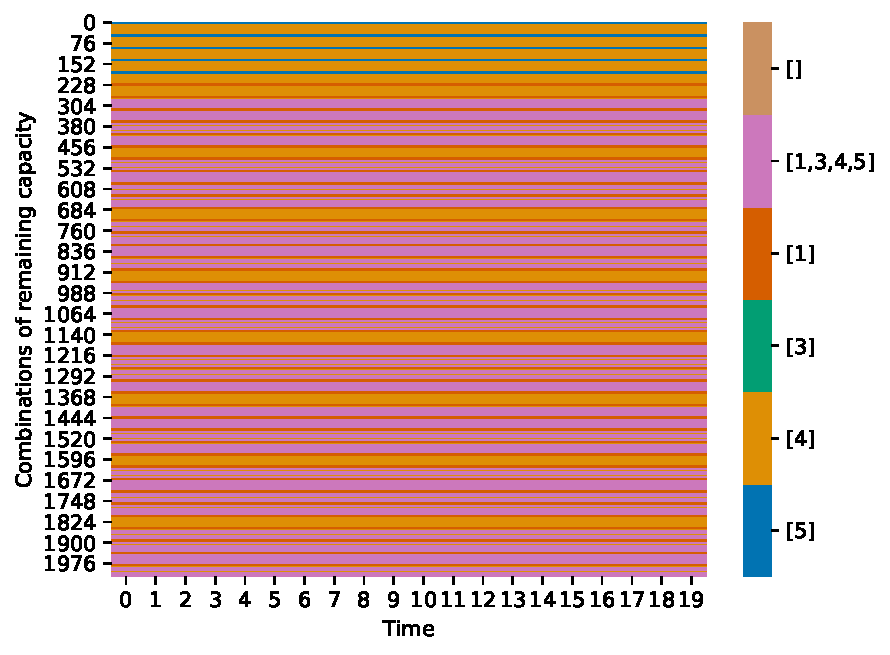
\includegraphics[width=\linewidth]{C:/Users/Stefan/LRZ Sync+Share/Masterarbeit-Klein/Code/Results/exampleStefan-True-APILinearMultiLeg-190918-1053/offersetsAll59.pdf}
		\caption{\label{fig-adp-offersets59} $k=59$}
	\end{subfigure}%
	\begin{subfigure}[t]{.5\textwidth}
		\centering
		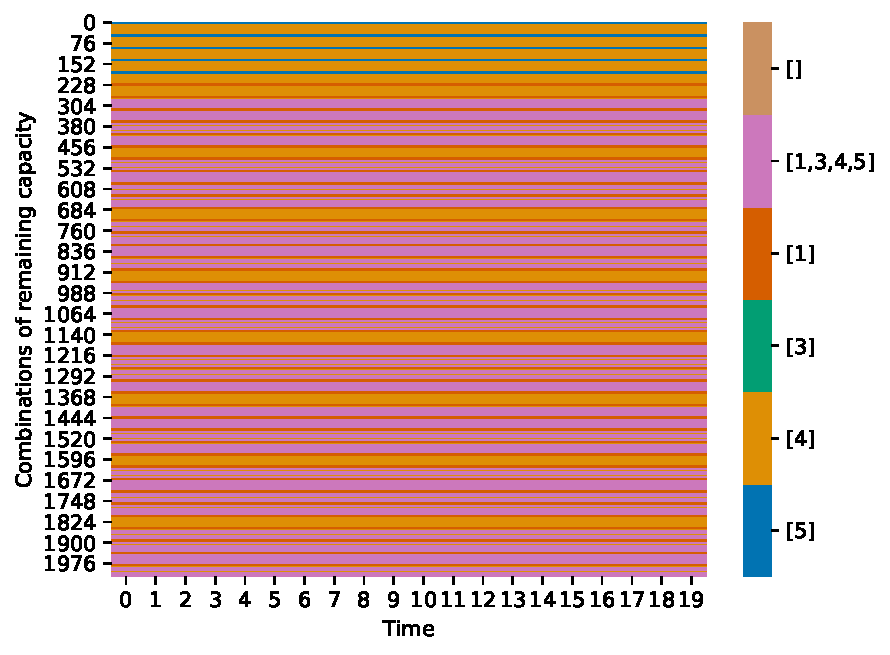
\includegraphics[width=\linewidth]{C:/Users/Stefan/LRZ Sync+Share/Masterarbeit-Klein/Code/Results/exampleStefan-True-APILinearMultiLeg-190918-1053/offersetsAll60.pdf}
		\caption{\label{fig-adp-offersets60} $k=60$}
	\end{subfigure}
	\caption[Categorical maps of offersets for all combinations of remaining capacity.]{\label{fig-adp-offersets}Categorical map of offersets for all combinations of remaining capacity for the two final policy iterations.}
\end{figure}